\documentclass[a4paper,fleqn]{cas-sc}
\usepackage[pagewise]{lineno}
\linenumbers

\usepackage[numbers]{natbib}
\usepackage{subfiles}
\usepackage[version=4]{mhchem}
\usepackage{cleveref}
\usepackage{subcaption}
\usepackage{longtable}
\usepackage{subcaption}
\usepackage{array}
\usepackage{mathtools} 
\usepackage{tabularx}
\usepackage{makecell}
\usepackage{tabularx}
\usepackage{booktabs}
\usepackage{adjustbox}
\usepackage{tabularx}
\usepackage{makecell}
\renewcommand\cellalign{tl}
\newcolumntype{P}[1]{>{\centering\arraybackslash}p{#1}}
\usepackage{listings}
\usepackage{xcolor}

\lstset{
  basicstyle=\ttfamily\small,
  numbers=left,
  numberstyle=\tiny,
  numbersep=5pt,
  backgroundcolor=\color{gray!10},
  frame=single,
  breaklines=true,
  postbreak=\mbox{\textcolor{red}{$\hookrightarrow$}\space},
  keywordstyle=\color{blue},
  commentstyle=\color{gray},
  stringstyle=\color{orange},
  showstringspaces=false
}


\newcommand{\Ha}{\text{Ha}}
\newcommand{\COtwo}{{\ce{CO2}}}
\newcommand{\HtwoO}{{\ce{H2O}}}
\newcommand{\MEA}{{\ce{MEA}}}
\newcommand{\MEAH}{\ce{MEAH+}}
\newcommand{\MEACOO}{{\ce{MEACOO-}}}
\newcommand{\HCOthree}{{\ce{HCO3-}}}
\newcommand{\Ntwo}{{\ce{N2}}}
\newcommand{\Otwo}{{\ce{O2}}}
\newcommand{\NtwoO}{{\ce{N2O}}}

\newcommand{\A}{\text{A}}
\newcommand{\B}{\text{B}}
\newcommand{\C}{\text{C}}
\newcommand{\D}{\text{D}}

\newcommand{\code}[1]{\texttt{#1}}

\newcommand{\liq}{\ell}
\newcommand{\vap}{v}

\usepackage{listings}
\usepackage{color}
\usepackage{siunitx}

\definecolor{dkgreen}{rgb}{0,0.6,0}
\definecolor{gray}{rgb}{0.5,0.5,0.5}
\definecolor{mauve}{rgb}{0.58,0,0.82}

\lstset{
    frame=tb,
    language=Python,
    aboveskip=3mm,
    belowskip=3mm,
    showstringspaces=false,
    columns=flexible,
    basicstyle={\small\ttfamily},
    numbers=none,
    numberstyle=\tiny\color{gray},
    keywordstyle=\color{blue},
    commentstyle=\color{dkgreen},
    stringstyle=\color{mauve},
    breaklines=true,
    breakatwhitespace=true,
    tabsize=3
}

\begin{document}

    \let\WriteBookmarks\relax
    \def\floatpagepagefraction{1}
    \def\textpagefraction{.001}

    % Short title
    \shorttitle{Absorption Column Modeling}

    % Short author
    \shortauthors{Polley et al.}

    % Main title of the paper
    \title [mode = title]{MEA Absorption Column Model Framework and Simulation Method Analysis}

    \author[1]{Tanner W. Polley}
    \author[2]{Tyler Garn}
    \author[3]{Douglas A. Allan}
    \author[4]{John D. Hedengren}

    % Email id of the first author
    % \ead{tannerwpolley@gmail.com}

    % Here goes the abstract
    \begin{abstract}
        Post-combustion carbon capture (PCC) using amine-based absorption is a critical technology for mitigating CO$_2$ emissions from industrial processes and power generation. Developing reliable and efficient models for this process is essential in facilitating the adoption of PCC technologies in industry by enabling cost-effective scaling, risk assessment, and integration into existing infrastructures. However, traditional models often face trade-offs between accuracy and computational speed, posing challenges for iterative testing and rapid decision-making. This study focuses on the development and evaluation of a fast yet sufficiently accurate model for amine-based absorption processes. Such models are crucial for performing iterative testing for parameter analysis or design optimization. Since run counts for these iterative tests can reach the thousands, a fast model with sufficient accuracy and robustness is required. The inherent complexity of these systems, which include coupled mass and energy balances alongside non-linear reaction kinetics and vapor-liquid equilibrium, also necessitates robust numerical methods for their solution. We analyze three prominent numerical techniques for solving these models: the shooting method, finite difference method, and collocation method. Through comparative analysis, this work highlights the trade-offs between accuracy, computational efficiency, and ease of implementation for each method. The findings underscore the importance of tailoring the numerical approach to the specific requirements of PCC modeling applications, balancing the need for speed and precision. Ultimately, this research aims to contribute to the development of practical tools for advancing the deployment of amine-based carbon capture systems, thus accelerating their industrial adoption and impact.
    \end{abstract}

    \begin{keywords}
        Numerical Methods \sep Python \sep Carbon Dioxide Capture \sep Modeling \sep MEA Absorption \sep Post-Combustion Carbon Capture \sep Process Simulation \sep
    \end{keywords}

    \maketitle

    \section{Introduction}\label{sec:introduction}
        Post-combustion carbon capture (PCC) has emerged as a leading approach for reducing CO\textsubscript{2} emissions, particularly in power plants and industrial facilities that rely on fossil fuels. Among the different PCC techniques, amine-based absorption is effective, mature, and relative easy to retrofit into existing infrastructure. However, designing, analyzing, and optimizing these systems is challenging because they involve complex, coupled phenomena such as vapor-liquid equilibrium, chemical reaction kinetics, and transport processes. Over the years, researchers have introduced various model formulations and numerical methods to capture the underlying physics, but a key hurdle remains balancing high-fidelity accuracy against computational efficiency. This tension is especially relevant when evaluating a range of operating conditions, as engineering teams increasingly depend on large sets of simulations (i.e., iterative runs) to explore design alternatives, perform risk assessments, or guide control strategies. Rapid and robust computational models become essential, both in academic investigations and industrial deployments. 
        
        This paper compares three prominent numerical methods (shooting, finite difference, and collocation) to find a modeling solution that efficiently captures the essential behavior of amine-based absorption columns. The model framework includes mass/energy balances and integrated transport and reaction kinetics. Each numerical method is described and a custom Python model demonstrates the strengths of each.  This custom model is used for robust parameter testing or input design tests that simulate runs in under 5 seconds with sufficient accuracy and validated with pilot plant results. The benchmarks from each method focus on factors such as computational time, accuracy, and sensitivity to parameter variations. Finally, the paper concludes with how this modeling framework, method comparison, and Python model can expedite future research on PCC technology, offering guidelines for striking a balance between speed and precision in large-scale iterative simulations. 

        \subsection{Literature Review}

        This literature review surveys past work on mechanistic models, various simulation methods, and uncertainty quantification efforts for amine-based systems, identifying gaps and motivations that inform this current study. A significant share of the literature focuses on the development of mechanistic and rate-based models that couple chemical kinetics with thermodynamic phase equilibria. Pioneering work by \citet{Freguia2003ModelingMonoethanolamine} provided a comprehensive mechanistic model that incorporated gas-liquid equilibrium and chemical reaction kinetics for CO$_2$ absorption into MEA. Their work forms the foundation of most modern rate-based modeling efforts, as it offers a robust framework for evaluating both equilibrium and rate-based models. Mores et al. \cite{Mores2012ASolution} built on this foundation by implementing a rate-based packed column model that combined detailed mass transfer kinetics and thermodynamic correlations. Their model enabled better prediction of CO$_2$ loading profiles and absorber performance across varying process conditions. Zhang et al. \cite{Zhang2009Rate-basedSolution} conducted one of the earliest comprehensive simulations using rate-based models, analyzing system sensitivity under operational constraints.
        
        Following the establishment of reliable thermodynamic models, research shifted toward process simulations. Moioli et al. (2012) \cite{Moioli2012SimulationModel} used rate-based modeling to simulate CO$_2$ capture via MEA scrubbing under different load and control scenarios. This work provided insights into operational flexibility and optimization techniques. Mohamadbigy et al. \cite{Mohamadbigy2005AmineSimulation} also explored the application of mass transfer rate simulations in designing MEA absorption columns, contributing to early-stage process design tools. Harun \cite{Harun2012DynamicPlants} developed dynamic simulations of MEA absorbers under power plant conditions, highlighting the significance of transient responses to fluctuations in flue gas composition and flow rates. Similarly, Greer (2008) \cite{Greer2008ModelingCapturing} focused on dynamic modeling frameworks aimed at absorber control strategy development for real-world applications.
    
        Model validation is critical for ensuring the accuracy and applicability of simulation results. Tobiesen (2007) \cite{Tobiesen2007} conducted experimental validation of rate-based MEA absorber models using pilot-scale plant data, reinforcing confidence in the simulation results. Razi et al. (2013) \cite{Razi2013ValidationData} also used pilot plant data to validate mass transfer correlations, refining kinetic and transport parameters for improved modeling accuracy. Shahid et al. (2019) \cite{Shahid2019} made substantial contributions by validating MEA models under high-pressure and high-CO$_2$ loading conditions, extending model applicability to more extreme industrial operating environments. Chinen et al. (2018) \cite{Chinen2018} advanced model robustness by integrating hydraulic and mass transfer modeling with uncertainty quantification frameworks.
    
        Given the variability of CO$_2$ emissions in real systems, dynamic modeling is essential. Kvamsdal et al. (2009) \cite{Kvamsdal2009DynamicCapture} presented a complete dynamic simulation of MEA absorber columns, including the effects of the temperature bulge and load variations. Their model became a benchmark for dynamic process studies. Akula et al. (2021) \cite{Akula2021a} extended this work by modeling MEA systems under part-load and variable operations. Their model introduced a flexible architecture adaptable to operational fluctuations in carbon capture. Akula (2022) \cite{Akula2022} further enhanced modeling efforts by developing optimization algorithms for amine-based carbon capture systems, aiming to improve process efficiency and reduce energy consumption. Supplementary modeling parameters and extended configurations provided in Akula (2021) \cite{Akula2021} allow replicability and deeper analysis.
    
        Innovation in absorber column internals has been another key area of research. Moore et al. (2021) \cite{Moore2021AdvancedPackings} investigated absorber heat integration using specially designed heat-exchange packings. Their findings suggest that integration can significantly improve energy efficiency and operational performance. Thompson and Tsouris (2021) \cite{Thompson2021Rate-BasedPacking} examined the application of additively manufactured structured packing in MEA absorbers, modeling its impact on pressure drop and mass transfer rates. Their work paves the way for future process intensification through advanced material design.
    
        The transition from laboratory to industrial-scale systems requires scalable modeling approaches. Olajide et al. (2020) \cite{Olajide2020} introduced a novel scale-up methodology for packed columns, facilitating efficient extrapolation from pilot to industrial systems. Thiels et al. (2016) \cite{Thiels2016ModellingColumn} contrasted traditional packed columns with rotating packed beds in MEA systems, providing performance metrics for intensified contactor designs. Restrepo et al. (2022) \cite{Restrepo2022DesignPlant} contributed by modeling and designing a lab-scale absorption tower, offering a benchmark for academic and pilot-scale implementation of MEA absorption technology.
    
        Several studies compared MEA with other solvent systems to benchmark modeling performance. Plaza et al. (2011) \cite{Plaza2011ModelingCommittee} used rigorous thermodynamic modeling to evaluate MEA, PZ, and promoted potassium carbonate blends. Kothandaraman (2010) \cite{AnushaKothandaramanChemEng2010CarbonStudy} evaluated multiple solvent options for CO$_2$ capture, positioning MEA as a baseline. Rodriguez et al. (2014) \cite{Rodriguez2014} developed an integrated framework for dynamic modeling of solvent-based CO$_2$ capture processes, of which MEA absorption was a core module. Saimpert et al. (2013) \cite{Saimpert2013ATool} created a generic modeling tool for absorbers and desorbers validated for MEA systems, enabling easier adaptation of models across solvent types.

    \subsection{Summary}
    
        In surveying the broad array of modeling efforts in amine-based PCC, it became evident that while many studies have tackled individual elements, such as mass transfer kinetics, thermodynamic equilibrium, or process dynamics, there is a lack of a single, unified, and relatively simple model framework that comprehensively integrates these aspects for an MEA absorption column. This framework would work as a conglomerate model that included every relevant and necessary component of the model. Numerous authors have proposed specialized or partial models, yet each tends to focus on specific features (e.g., reaction mechanism, transport, or scale-up), often leading to fragmented findings when trying to capture the entire process flow. Moreover, although there are ample accounts of how individual simulation methods to perform on certain subsets of problems, systematic comparisons of multiple numerical techniques applied to a single, clearly defined model are not commonly found in the literature. As a result, both a coherent model that faithfully represents all major phenomena in an MEA-based absorber and a side-by-side assessment of different solution methods remains a significant gap that this work aims to address.
    

    \section{Model Framework}
        Solvent-based PCC models are built to replicate the absorption phenomena occurring in industrial-packed columns. The dimensions of an absorption column have a certain height and diameter that are scaled on the demand of the input streams of liquid and vapor. The absorption phenomenon occurs when the thermodynamic driving force for $\COtwo$ is pushed from vapor to liquid. This driving force and the speed at which it happens are dependent on multiple factors such as transport, vapor-liquid equilibrium, and the kinetics of the reaction occurring. Accounting for all of these and their interactions together is key to solving this model. Each of these is also dependent on the properties of each stream and element found in the system which are typically dependent on the temperature and composition of the streams. These variables are tracked by the governing equations seen as the mass and energy balances of the system. These governing equations are found as differential equations and solving these is key to simulating the column.

        \begin{figure}[ht]
            \centering
            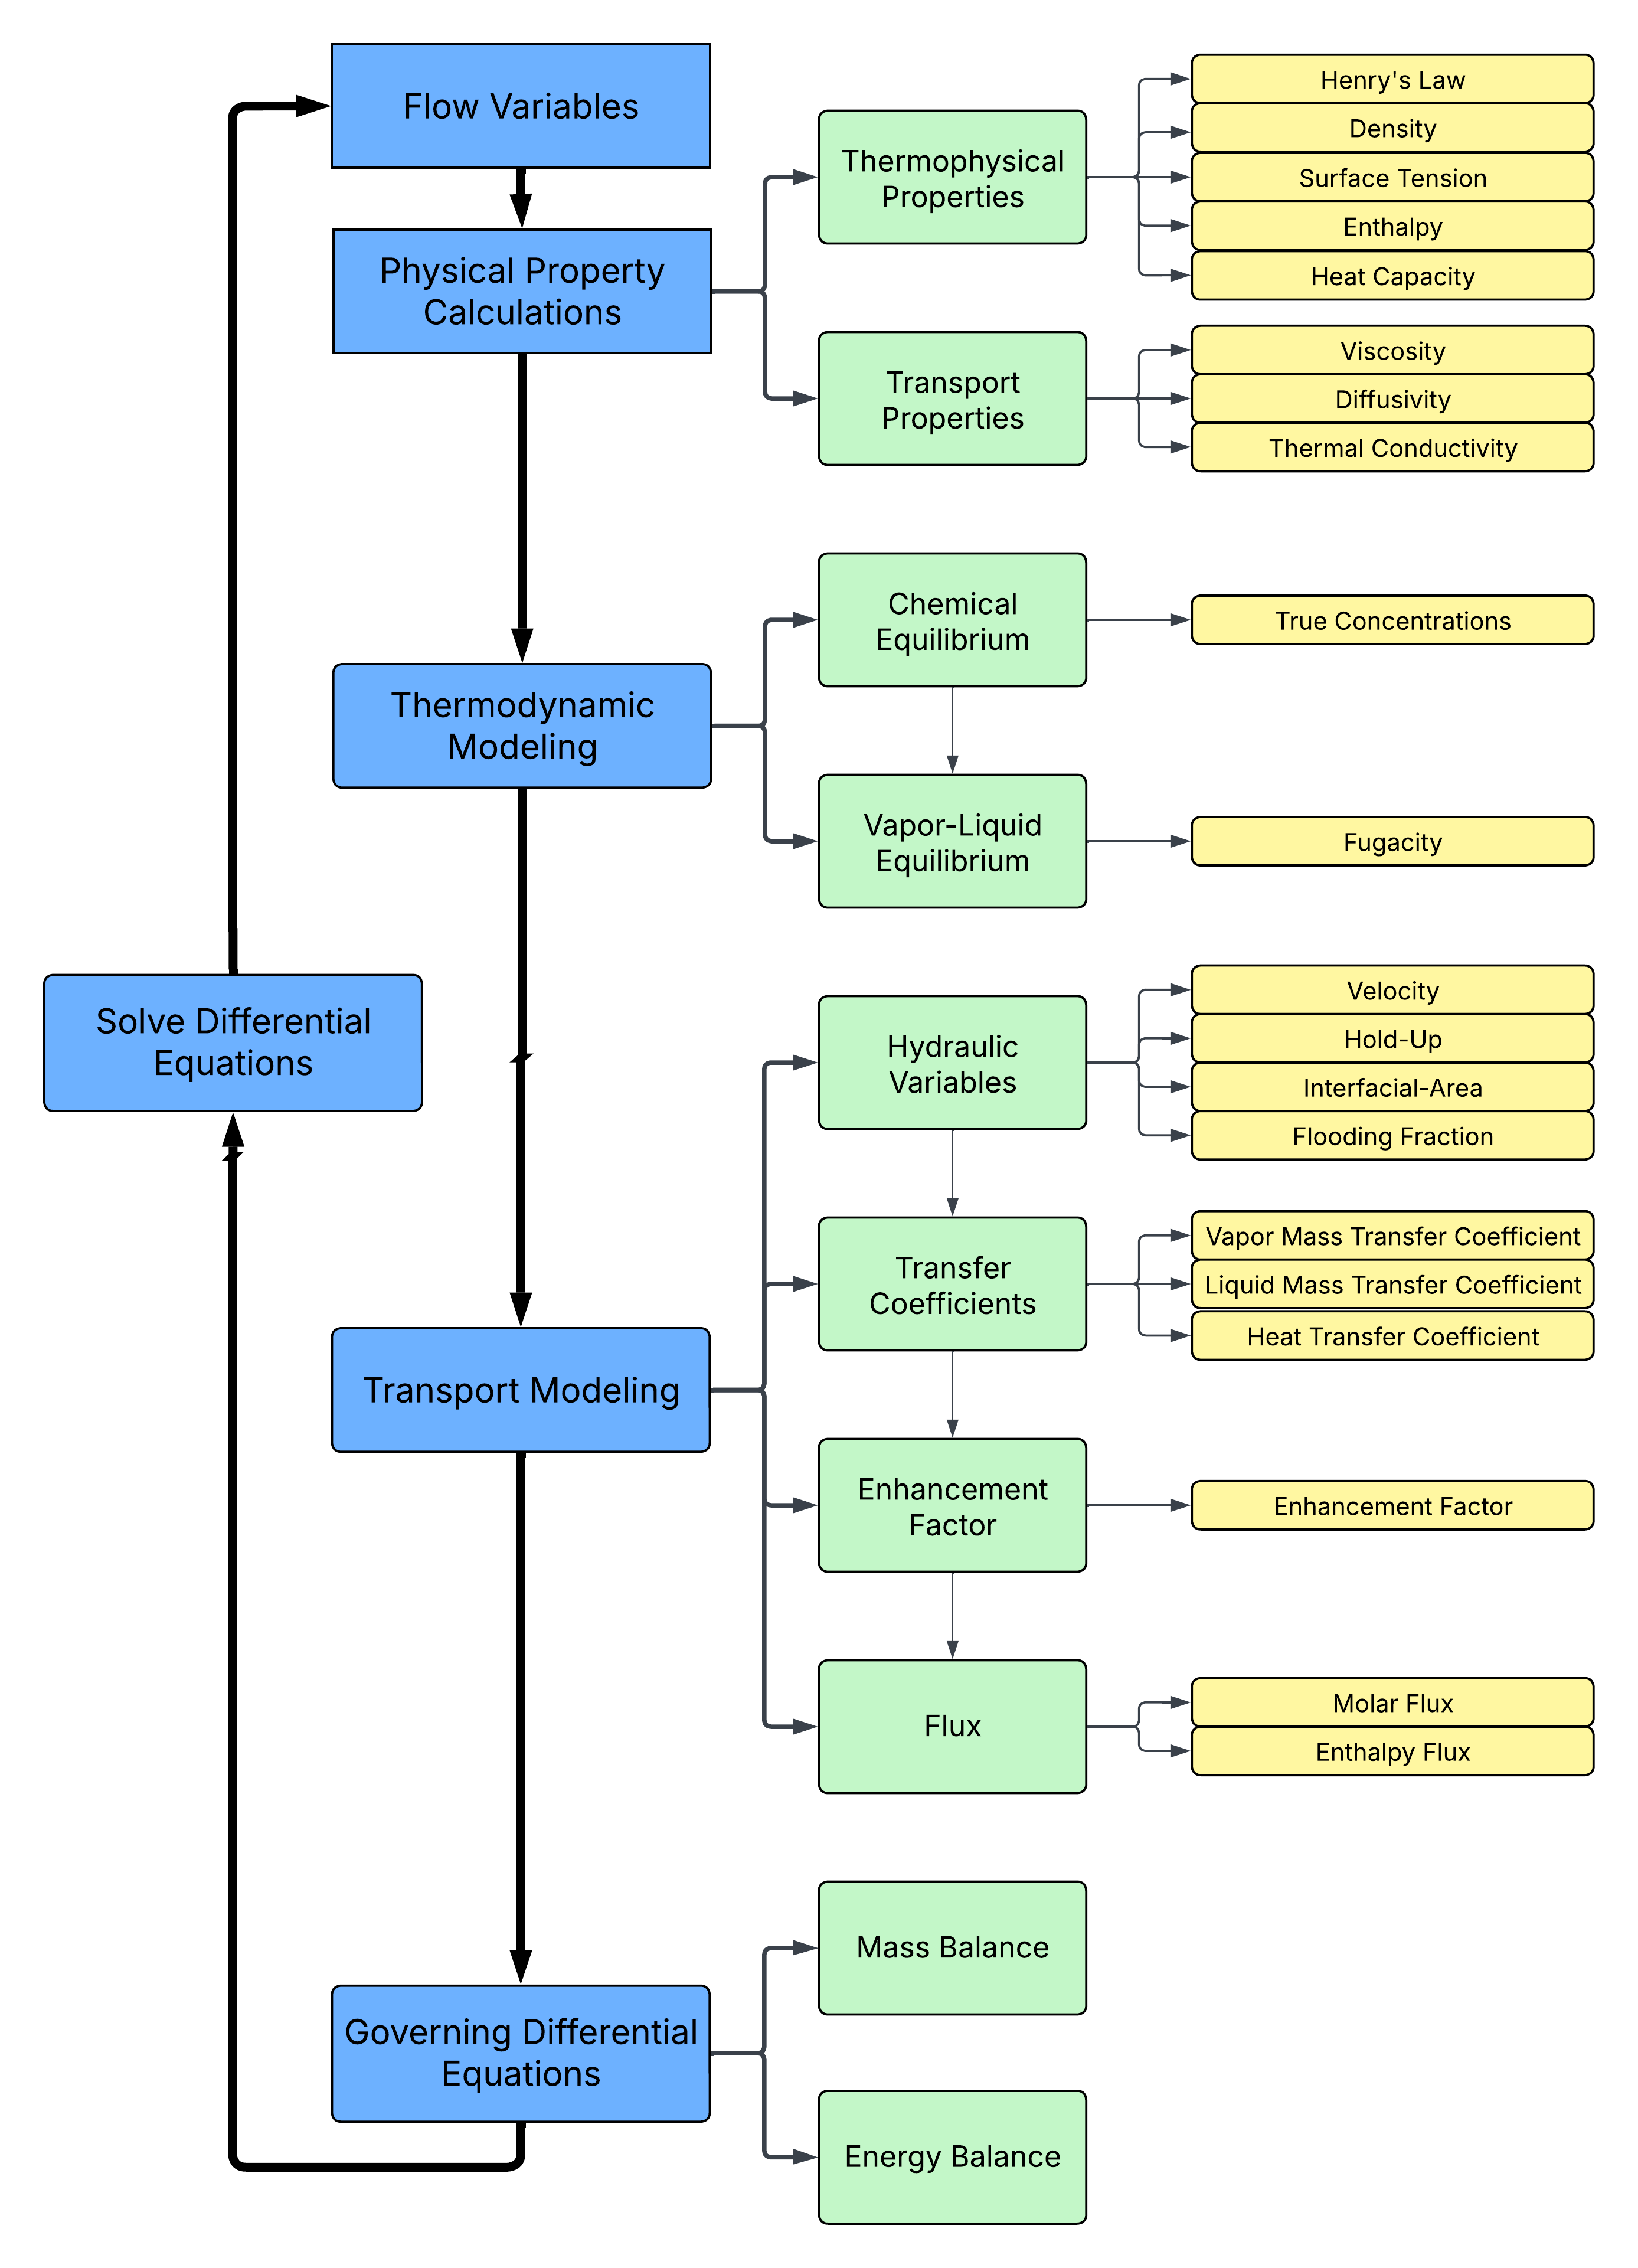
\includegraphics[width=12cm]{figs/Model_Framework_Flowchart.png}
            \caption{Model Framework}\label{fig:Model_Framework_Flowchart}
        \end{figure}
        The diagram in Figure~\ref{fig:Model_Framework_Flowchart} inspired from Luo \cite{Luo2017ImprovingDeployment} outlines the complete 
        model framework developed for simulating the amine-based absorption column model 
        used in post-combustion $\COtwo$ capture. It begins with the specification of flow variables, such as flow rates, compositions, and temperatures for both vapor and 
        liquid phases. These flow variables are the design variables that the solver, whichever method, is estimating to converge onto the solution and match the boundary conditions. These variables are first used to calculate all physical property calculations, which is divided into thermophysical and transport 
        properties. Thermophysical properties include Henry’s law constants, density, surface tension, enthalpy, and heat capacity, while transport properties encompass viscosity, diffusivity, and thermal conductivity. These properties are critical for capturing the physical behavior of the system and are used extensively in both thermodynamic and transport modeling.
        
        Thermodynamic modeling follows, incorporating both the chemical equilibrium and vapor-liquid equilibrium (VLE) of the model. The chemical equilibrium determines the true species concentrations based on the reaction set and apparent mole fractions and its results are quite sensitive to the overall stability and results of the model. The VLE computes the fugacity of the species, the key thermodynamic driving force. The model is setup to be able to switch to any VLE model given, be it an idealized model utilizing only Henry's solubility laws, an activity coefficient such as NRTL, or an equation of state model like ePC-SAFT \cite{Cameretti2005ModelingOriginal}. A comparison of these models is very relevant to amine-based absorption column simulations but is set for future work. Once the thermodynamics is evaluated, it is utilized alongside most of the properties in determining the transport phenomena of the model which contains hydraulic variables (e.g., velocity, holdup, interfacial area), transfer coefficients (e.g., mass and heat transfer), and an enhancement factor to quantify reaction-driven mass transfer. All these components, along size the fugacity differential, feed into the calculation of species fluxes, both molar and enthalpic, which in turn define the governing differential equations. These include mass and energy balances, which are numerically solved to predict the column's performance. Once the solver approximates the differential equations congruent with the boundary conditions, a new set of design variables are tested and sent back to the model framework. 

        \subsection{Thermodynamics}\label{subsec:thermodynamics}
            The thermodynamics section of the model establishes the chemical and phase behavior that drives $\COtwo$ absorption in the MEA solvent system. It begins with solving chemical equilibrium by determining the true species concentrations. Once the true concentrations are known, vapor–liquid equilibrium is modeled to determine the fugacities of the species. Together, the chemical equilibrium and VLE models provide the thermodynamic foundation for accurately predicting mass transfer and absorption behavior throughout the column.
        
            \subsubsection{Chemical Equilibrium}
                Solving for the chemical equilibrium of the liquid solvent is a key first step in solving for the absorption. Upon solving for the chemical equilibrium, the concentration of the true species are found which are used throughout the rest of the model both in the thermodynamics and transport correlations. The methodology to solve for the true species begins with the concentration of the apparent species and equilibrium constants for the two main reactions found.
                \begin{align}
                    & 2 \MEA+\COtwo \leftrightarrow \MEAH +\MEACOO- \\
                    & \MEA+\COtwo+\HtwoO \leftrightarrow \MEAH +\HCOthree
                \end{align}
                This reaction set represents a simplification of the solution chemistry that was developed by Hilliard \cite{Hillard2008} for typical $\COtwo$ capture process conditions where concentrations of other ions (${\text{H}_3 \text{O}}^+$,${\text{OH}}^-$,${\text{CO}_3}^{2-}$ ) are negligibly low. 

                This reaction set leads to the following stoichiometric matrix $\mathbf{\nu}_{r,i}$ is then  
                \begin{align}
                    \mathbf{\nu}_{i, r} = 
                    \begin{bmatrix}
                    -1 & -1 \\
                    -2 & -1 \\
                     0 & -1 \\
                     1 &  1 \\
                     1 &  0 \\
                     0 &  1
                    \end{bmatrix}
                \end{align}
                The equilibrium constants are found through fitting speciation data to the following equation.
                
                \begin{align}
                    \log K_r = a_r + \frac{b_r}{T_l} + c_r \ln(T_l) + d_r T_l
                \end{align}

                 Where $r$ represents a reaction number. 
                 
                 The reaction quotient in terms of concentration is the following. 
                 
                 \begin{align}
                    Q_r &= \prod_i \text{C}_i^{\nu_{i,r}}
                 \end{align}
                 wherefore the relationship
                 \begin{align}
                    Q_r &= K_r
                \end{align}
                is utilized for both reactions and used in the system of equations alongside the material and charge balance equations which are derived from Akula \cite{Akula2023AppendixAkula}.

                \begin{align}
                    C^{\liq}_{\ce{CO2},0} &= C^{\liq}_{\ce{CO2}} + C^{\liq}_{\ce{MEAH}^{+}} \\
                    C^{\liq}_{\ce{MEA},0} &= C^{\liq}_{\ce{MEA}} + C^{\liq}_{\ce{MEAH}^{+}} + C^{\liq}_{\ce{MEACOO}^{-}} \\
                    C^{\liq}_{\ce{H2O},0} &= C^{\liq}_{\ce{H2O}} + C^{\liq}_{\ce{MEAH}^{+}} - C^{\liq}_{\ce{MEACOO}^{-}} \\
                    C^{\liq}_{\ce{MEAH}^{+}} &= C^{\liq}_{\ce{MEACOO}^{-}} + C^{\liq}_{\ce{HCO3}^{-}} \\
                    \textbf{C} &= \left[
                         C^{\liq}_{\COtwo}, C^{\liq}_{\MEA}, C^{\liq}_{\HtwoO}, C^{\liq}_{\MEAH}, C^{\liq}_{\MEACOO}, C^{\liq}_{\HCOthree}\right]
                \end{align}
                Where $\textbf{C}$ is the array of unknowns as the concentration of true species.
                Each equation is then set equal to zero and utilizing a non-linear solver, the true species concentration is found via the roots of the non-linear system of equations. Concentration was chosen as the variable used since this model currently assumed that the activity coefficient of each species is one and concentration is larger in value that mole fraction. Since the true mole fraction of $\COtwo$ can get quite small near near the top of the column, scaling for both the unknowns and each equation is pivotal in allowing the root-finder to converge. Generous initial guesses are also necessary due to the non-linearity of the equations. A technique of utilizing a python functions own attribute to store the previous iterations result in order to use this result as the next iterations guess was utilized. This method proved reliable and efficient, with Newton’s method consistently converging at the column base when $x_{\COtwo, true}$ is larger and will continue to use each result step-wise as it solves up the column.This omitted the need to of having a surrogate model predict the array of initial guesses depending on the current height of the column or apparent mole fractions and temperatures. Another option is to use extent of reactions $(\xi)$ and minimize $\Delta _{rxn} G^{\circ}$ to initialize a set of guesses. Fortunately the previous method was deemed adequate and can save on computational time. Once true species concentrations are known, VLE behavior can be evaluated.


            \subsubsection{Vapor-Liquid Equilibrium}
                The vapor-liquid equilibrium of the model is what determines the driving force of the $\COtwo$ absorption that occurs within the column. This driving force is the difference between the vapor and liquid fugacities of $\COtwo$. Significant progress has been made in developing accurate models for phase behavior. Of the most sophisticated is the e-NRTL activity coefficient model originally developed by Zhang at el. \cite{Zhang2011ThermodynamicModel}. In this model, binary electrolyte interactions parameters between molecules and electrolytes are fit with speciation data and many thermodynamic expressions are derived such as heat capacity and excess enthalpy. This model has shown to predict the $\MEA-\HtwoO-\COtwo$ system very well. The only draw back is the amount of parameters required and the complexity of the model, which can be a hindrance to the convergence of the model when running numerous simulations for statistical testing. Other models such as the ePC-SAFT equation of state model are rather new in the field of amine-based absorption and has shown to be promising to reduce the number of required parameters and complexity without losing the required accuracy. Though for this model, a simpler VLE model was chosen in order to maximize the speed and stability of the model since its main objective is running numerous simulations for statistical analysis/uncertainty quantification. The simplified model incorporates complexity into Henry’s Law, using regressed parameters to capture key interactions. The following outlines the derivation and assumptions for relating liquid fugacity to Henry’s Law. First start with the definition of equilibrium for a species between two phases (liquid, vapor):
                \begin{equation}
                    f_i^v = f_i^l
                \end{equation}
                
                Evaluate both fugacities in terms of fugacity/activity coefficients:
                \begin{equation}
                    y_i \, \hat{\phi}_i^v \, P = x_i \, \gamma_i \, f_i^\circ
                \end{equation}
                
                If $i$ is an infinitely dilute solute such that:
                \begin{equation}
                    \lim_{x_i \to 0} \left( \frac{f_i^l}{x_i} \right) = H_{i,j}
                \end{equation}
                
                Then $f_i^l = x_i H_{i,j} = x_i$, and therefore $H_{i,j} = \gamma_i \, f_i^\circ$, and we can substitute this in and assume ideal gas for the vapor phase to get:
                \begin{equation}
                    y_i\, P = x_i H_{i,j}
                \end{equation}
                
                We can then change Henry's Law into concentration form:
                \begin{equation}
                    y_i \, P = C_i \, H^{c}_{i,j}
                \end{equation}
                
                Therefore, we obtain the simplified expressions:
                \begin{align}
                    f_i^v &= y_i P \\
                    f_i^l &= C_i H^{c}_{i,j}
                \end{align}

                If using an activity coefficient model, then Henry's Law is also used to determine the activity coefficient of the solute ($\COtwo$) through the infinitely dilute activity coefficient $H_{i,j} = \gamma^{\infty}_i f^{\circ}_i$.
                
                The following equations summarize the equations used in the model for the fugacity of $\COtwo$.
                \begin{align}
                    \textit{f}^{\:\vap}_{ \COtwo} &= P y_{\COtwo} && \left(\unit{Pa} \right)\\
                    \textit{f}^{\:\liq}_{ \COtwo} &= C^{\liq}_{ \COtwo, \text{true}} H_{\COtwo,\text{mix}} &&\left(\unit{Pa} \right) \label{eq:ideal}
                \end{align}
                The parameters used to determine the Henry's Law expression for $\COtwo$ in the liquid mixture are specifically tuned to account for as many interactions as possible and are fitted with speciation data. Unfortunately, this method has the drawback of less potential accuracy compared to a more rigorous model such as e-NRTL activity coefficient model or ePC-SAFT equation of state model. With less rigor, though, brings much more stability and consistency, which is important when attempting to run a model for many simulations. 
                The following equations for the fugacity of $\HtwoO$ are below
                \begin{align}
                    \textit{f}^{\:\vap}_{ \HtwoO} &= P y_{\HtwoO} && \left(\unit{Pa} \right)\\
                    \textit{f}^{\:\liq}_{ \HtwoO} &= P_{\text{sat}, \HtwoO} x_{\HtwoO, \text{true}} && \left(\unit{Pa} \right)
                \end{align}
                and these equations are sufficiently accurate since $\HtwoO$ is the abundant solvent in this liquid mixture and can assume $\gamma_{\HtwoO} = 1$. These fugacities play an important role in the water balance of the column which largely dictates the energy balance and temperature behavior within the column. The differential in fugacity between the vapor and liquid phases represents the thermodynamic driving force for mass transfer, quantifying the imbalance between the phases. When the fugacities are unequal, the system is not at equilibrium, and the magnitude of this difference indicates how far the system is from reaching equilibrium. Alongside the driving force, the transport phenomena, specifically the transfer coefficients, is needed to complete the full picture of the $\COtwo$ absorption.

        \subsection{Transport}\label{subsec:transport}
            The transport properties govern the flow of overall substance within the column. Of the properties, the mass transfer coefficients are terms that quantify the resistance of transfer that each species has between the proposed barrier. This resistance is quantified with the dimensions of the column, the type and size of the packing, and the properties of the liquid and vapor mixtures. Each of the relevant properties is found using the temperature and composition as inputs and a functional correlation with tuned parameters. The relevant properties used are density, viscosity, diffusivity, and surface tension. These properties will be covered later in the paper. Within transport, you can differentiate between the two types of transfer, mass-transfer and heat-transfer. Accurate $\COtwo$ flux prediction depends on modeling mass transfer effectively. The heat-transfer component plays a role in the energy balance between the two phases present in the column

            \subsubsection{Hydraulic Variables and Correlations}
                \paragraph{Velocity}\mbox{}\\[0.5em]
                The velocities of each phase are a simple derivation from molar flow rate and density
                \begin{align}
                    u_l &= \frac{F^{\liq}_{T}}{A \,\rho^{\liq}_{ \text{mol}}} \\
                    u_v &= \frac{F^{\vap}_{T}}{A \,\rho^{\vap}_{ \text{mol}}}.
                \end{align}

                \paragraph{Inter-facial Area}\mbox{}\\[0.5em]
                The interfacial area is the area in which the transfer happens and is dependent on the density, surface tension, and a packing constant. It is found both in the final molar flux equation as well as a part of the mass transfer coefficients given by Tsai~\cite{Tsai2010}.
                \begin{align}
                    a_e 
                    &= 1.42\,a_p\left[\frac{\rho_L}{\sigma_L}\,g^{1/3}\left(\frac{u_L}{a_p}\right)^{4/3}\right]^{0.116} && \left(\frac{\unit{m}^2}{\unit{m}^3} \right)
                \end{align}

                \paragraph{Liquid Holdup}\mbox{}\\[0.5em]
                The liquid holdup is the volume of liquid held per volume of a packed bed under operating conditions. It is found in each of the mass transfer coefficient equations given by Chinen and Tsai~\cite{Chinen2018,Tsai2010}
                \begin{align}
                    h_L &= A\left[u_L \alpha\left(\frac{\mu_L}{\rho_L}\right)^{1 / 3}\right]^{B} && \left(\unit{m}^3 \right)\\
                    h_V &= \epsilon - h_L && \left(\unit{m}^3 \right)
                \end{align}
                Where $A$ and $B$ are correlation parameters $\alpha$ is a parameter that combines multiple packing-specific constants

                \paragraph{Mass Transfer Coefficients}\mbox{}\\[0.5em]
                The mass transfer coefficients for vapor and liquid depend on several components such as densities, viscosities, surface tension, flow velocities, specific surface area, void fraction, and other packing-specific constants. These constants are found through regression with a large database for multiple types of packing and sizes by Billet and Chinen\cite{Billet1999, Chinen2018}.
                \begin{align}
                    k_l &= C_L \cdot 12^{1 / 6}\left(\frac{u_L}{h_L}\right)^{1 / 2}\left(\frac{D_L}{d_h}\right)^{1 / 2} && \left(\frac{\unit{m} }{\unit{s}} \right)\\
                    k_v &= \frac{C^{\vap}\,D^{\vap}\,RT_v}{}
                           \left(\frac{a_p}{d_h\,h_V}\right)^{1/2}  
                           \left(\frac{u^{\vap}}{\rho^{\vap}\,a_p\,\mu^{\vap}}\right)^{3 / 4}
                           \left(\frac{\mu^{\vap}}{\rho^{\vap}}\,D^{\vap}\right)^{1 / 3}
                           && \left(\frac{\unit{mol} }{\unit{Pa} \cdot{m}^2 \cdot \unit{s}} \right)
                \end{align}

                \paragraph{Heat Transfer Coefficient}\mbox{}\\[0.5em]
                Here is the overall heat transfer coefficient formulated by the Chilton-Colburn analogy
                \begin{align}
                    U_T = \left(\frac{(k^{\vap}_{\COtwo}\,P)^3\,{k_{t}^{\vap}}^{2}\,C^{\vap}_{p,T}}{\rho^{\vap}_{\text{mol}}\,{D^{\vap}_{\COtwo}}^2}\right)^{\frac{1}{3}}
                \end{align}

                \paragraph{Enhancement Factor}\mbox{}\\[0.5em]
                The enhancement factor is defined as the ratio of mass transfer from chemical absorption compared to physical absorption. It is therefore a relative factor which indicates the improvements of a reactive solvent compared to a physical non-reactive solvent. The enhancement factor is preferred in process simulations since it reduces the computational load. The chosen model to compute the enhancement factor comes from Gaspar\cite{Gaspar2015} which is solved by solving a system of two non-linear equations. The following equations can be defined outside the non-linear system of equations
                \begin{align}
                    k_2 &= 3.1732 \times 10^{9} \exp\left( \frac{-4936.6}{T_l}\right) \\
                    Ha &= \frac{\sqrt{k_2 C^{\liq}_{\MEA,true} D^{\liq}_{\COtwo}}}{k^{\liq}_{\COtwo}}
                \end{align}
                $k_2$ is the rate of the chemical reaction that governs the consumption of $\MEA$. $\text{Ha}$ is the Hatta number which compares the rate of reaction in a liquid film to the rate of diffusion through the film. The following equations are intermediate expressions contained within the system of equations that are dependent on $E$ and $\Upsilon_{\COtwo}.$
                \begin{align}
                    \Psi &= \frac{E \frac{k^{\liq}_{ \COtwo}}{k^{\vap}_{ \COtwo}}}{E \frac{k^{\liq}_{ \COtwo}}{k^{\vap}_{ \COtwo}} + H_{\COtwo, \text{mix}}} \\
                    C^{\liq,*}_{ \COtwo} &= \frac{\frac{y_{\COtwo}P}{\Psi} + C^{\liq}_{ \COtwo, true}}{\frac{H_{\COtwo,\text{mix}}}{\Psi} + 1}
                \end{align}
                $\Psi$ represents the overall correction factor for the driving force of $CO_2$ due to the Henry's Law and the present reactions. $C^{\liq, *}_{ \COtwo}$ is the liquid concentration of $CO_2$ at the interface.
                \begin{align}
                    \Upsilon_{\COtwo}^b &= \frac{C^{\liq}_{ \COtwo, true}}{C^{\liq,*}_{ \COtwo}} \\
                    \Upsilon_{\MEAH} &= 1+D^{\liq}_{ \MEA} {C^{\liq}_{\MEA, true}}\frac{1 - \Upsilon^{*}_{\MEA}}{2 D^{\liq}_{ \MEAH} C^{\liq}_{ \MEAH, true}} \\
                    \Upsilon_{\MEACOO} &= 1+D^{\liq}_{ \MEA} {C^{\liq}_{\MEA, true}}\frac{1 - \Upsilon^{*}_{\MEA}}{2 D^{\liq}_{ \MEACOO} C^{\liq}_{ \MEACOO, true}} \\
                    \Upsilon_{\COtwo}^{*} &= \frac{\Upsilon^{b}_{\COtwo} \Upsilon_{\MEAH} \Upsilon_{\MEACOO}}{{\Upsilon_{\MEA}}^{2}}
                \end{align}
                These equations represent dimensionless concentration quantities for each relevant species at bulk or interface
                \begin{align}
                    E_{\infty}^{*} &= 1+\frac{D^{\liq}_{\MEA} C^{\liq}_{\MEA, \text{true}}}{2 D^{\liq}_{ \COtwo} C^{\liq}_{ \COtwo, \text{true}}}
                \end{align}
                While $E_{\infty}^*$ is the instantaneous enhancement factor. The following equations constitute the governing equations for the two-equations-two-unknowns system.
                \begin{align}
                    E &= 1+\left(E_{\infty}^*-1\right) \frac{\left(1-\Upsilon_{\MEA}\right)}{\left(1-\Upsilon_{\COtwo}^b\right)} \\
                    E &= Ha \sqrt{\Upsilon_{\MEA}} \frac{1-\Upsilon_{\COtwo}^*}{1-\Upsilon_{\COtwo}^b}
                \end{align}
                A simple root solving method can obtain $E$ and can then obtain $\Psi_H$ to use in correcting the driving force of $\COtwo$
                \begin{align}
                    \Psi &= E \frac{k^{\liq}_{ \COtwo}}{k^{\vap}_{ \COtwo}} \\
                    \Psi_H &= \frac{\Psi}{\Psi + H_{\COtwo, \text{mix}}}
                \end{align}

            \subsubsection{Flux}
                \paragraph{Molar Flux}\mbox{}\\[0.5em]
                As shown above, the governing equations are composed of the molar flux of each corresponding species at the phase interface. Quantifying the molar flux is paramount in accurately accounting for the amount of species being transferred from one phase to the other.
                \begin{align}
                    N^{\vap}_{ \COtwo} &=  -k^{\vap}_{ \COtwo}  a_e A  \left(\textit{f}^{\:\vap}_{ \COtwo} - \textit{f}^{\:\liq}_{ \COtwo}\right) \Psi _{H} && \left(\frac{\unit{mol}}{\unit{s\cdot m}} \right) \\
                    N^{\liq}_{ \COtwo} &= -N^{\vap}_{ \COtwo} && \left(\frac{\unit{mol}}{\unit{s\cdot m}} \right) \\
                    N^{\vap}_{ \HtwoO} &= -k^{\vap}_{ \HtwoO} a_e A \left(\textit{f}^{\:\vap}_{ \HtwoO} - \textit{f}^{\:\liq}_{ \HtwoO}\right)  && \left(\frac{\unit{mol}}{\unit{s\cdot m}} \right) \\
                    N^{\liq}_{ \HtwoO} &= -N^{\vap}_{ \HtwoO} && \left(\frac{\unit{mol}}{\unit{s\cdot m}} \right)
                \end{align}
                Here flux is defined as a material flux $\left(\frac{\unit{mol}}{\unit{s\cdot m}} \right)$ and is in terms of length rather than area because the interfacial area of the specific packing material truncates the transfer onto the packed element rather than across the whole cross-sectional area of the column. For the flux equations, they are constituted with transport and thermodynamic components, while $\COtwo$ has an additional kinetic component. The transport components consist of the mass-transfer coefficients $\left(k_{j, i} \right)$, interfacial area $\left(a_e\right)$, and cross sectional area $\left(A\right)$. The thermodynamics involved conduct the driving force of the flux which is derived from the fugacity differential between the two phases. Since $\COtwo$ undergoes a reaction once it is absorbed in the liquid phase, a kinetic enhancement factor $\left(\Psi _{H}\right)$ is used to correct for this phenomena.

                \paragraph{Enthalpy Flux}\mbox{}\\[0.5em]
                The enthalpy flux is the sum of the enthalpy (chemical) and heat (conduction and convection) that is transferred across the interface. There is also a general heat transfer between the two phases where the driving force is the temperature gradient and is contained by the overall heat transfer coefficient $U$.
                \begin{align}
                    q^{\vap} &= -U a_e A \left(T_v-T_l\right) && \left(\frac{\unit{J}}                    {\unit{s\cdot m^2}} \right) \\
                    q^{\liq} &= -U a_e A \left(T_l-T_v\right) && \left(\frac{\unit{J}}                    {\unit{s\cdot m^2}} \right) \\
                    \dot{H}^{\vap}_{flux} &=   N^{\vap}_{ \COtwo}H^{\vap}_{ \COtwo} + N^{\vap}_{ \HtwoO}H^{\vap}_{ \HtwoO} +  q^{\vap} && \left(\frac{\unit{J}}{\unit{s\cdot m^2}} \right) \\
                    \dot{H}^{\liq}_{flux} &= N^{\liq}_{ \COtwo}H^{\liq}_{ \COtwo} + N^{\liq}_{ \HtwoO}H^{\liq}_{ \HtwoO} +  q^{\liq} && \left(\frac{\unit{J}}{\unit{s\cdot m^2}} \right)
                \end{align}

                The enthalpy transferred is the product of the molar enthalpy and molar flux of the transferring species ($\COtwo, \HtwoO$). There is also a heat transfer governed by the overall heat transfer coefficient $U$, interfacial $\left(a_e\right)$ and cross-sectional areas $\left(A\right)$, and the temperature gradient.
                
        \subsection{Governing Equations}\label{subsec:governing-equations}
            The governing equations are the backbone of the model. These equations are the culmination of the absorption phenomena and entail all aspects of the thermodynamics, transport, and kinetics of the model. In order to simulate the model, these differential equations are approximated via numerical methods such an a Runge-Kutta method, finite difference, or via collocation. The result of these approximations aid the solver to determine the next set of design variables to choose and then test in the absorption column framework and the iterative process will only conclude until sufficient tolerance is achieved.

            \subsubsection{Material Balance}\label{subsubsec:material-balance}
                The material balances are accounted for by molar flow $\left(F_{j, i}\right)$ which equate to the interfacial molar flux $\left(N_{j,i}\right)$. The flux moves across the interfacial phase boundary found on the packed elements within the column.
                \begin{align}
                    \frac{d F^{\liq}_{ \COtwo}}{d z} &= -N^{\liq}_{ \COtwo} && \left(\frac{\unit{mol}}{\unit{s\cdot m}} \right)\\
                    \frac{d F^{\liq}_{ \HtwoO}}{d z} &= -N^{\liq}_{ \HtwoO} && \left(\frac{\unit{mol}}{\unit{s\cdot m}} \right)\\
                    \frac{d F^{\vap}_{ \COtwo}}{d z} &= N^{\vap}_{ \COtwo} && \left(\frac{\unit{mol}}{\unit{s\cdot m}} \right)\\
                    \frac{d F^{\vap}_{ \HtwoO}}{d z} &= N^{\vap}_{ \HtwoO} && \left(\frac{\unit{mol}}{\unit{s\cdot m}} \right)
                \end{align}
                We can assume that the flow rates of $\MEA$, $\Ntwo$ and $\Otwo$ are steady-state through the column since the flux for these species across the phase boundary is negligible. Though flow rates are being accounted for in the differential equations, the more convenient form of mole fractions is used in the model and can be easily converted from flow rates.
                \begin{align}
                    x_i &= \frac{F^{\liq}_{ i}}{F^{\liq}_{ T}} \\
                    y_i &= \frac{F^{\vap}_{ i}}{F^{\vap}_{ T}} \\
                    \alpha &= \frac{x_{\COtwo}}{x_{\MEA}}
                \end{align}

            \subsubsection{Energy Balance}\label{subsubsec:energy-balance}
                The energy balances are similar to the material balances but instead of accounting for molar flow, it is enthalpy flow ($\dot{H}^{j}_{flux}$), and thus are governed by enthalpy flux ($\dot{H}_{j, flux}$) across the interfacial phase boundary.
                \begin{align}
                    \frac{d \dot{H}^{\liq}}{d z} &= \dot{H}^{\liq}_{flux} && \left(\frac{\unit{J}}{\unit{s\cdot m}} \right)\\
                    \frac{d \dot{H}^{\vap}}{d z} &= \dot{H}^{\vap}_{flux} && \left(\frac{\unit{K}}{\unit{s\cdot m}} \right)
                \end{align}
                You can also derive the temperature-based energy balances from these equations through the following derivation:
                Start with the overall energy balance based on enthalpy flow:
                \begin{equation}
                    \frac{d\dot{H}^j}{dz} = \dot{H}^{j}_{flux}
                \end{equation}
                
                Separate enthalpy flow into molar enthalpy and molar flow rate and use the product-rule:
                \begin{align}
                    \frac{d}{dz}(F^j H^j) &= \dot{H}^{j}_{flux} \\
                    \frac{dF^j}{dz} H^j + F^j \frac{dH^j}{dz} &= \dot{H}^{j}_{flux}
                \end{align}
                
                Now use chain-rule to convert the enthalpy differential to the temperature differential:
                \begin{equation}
                    \frac{dH^j}{dz} = \frac{dH^j}{dT^j} \cdot \frac{dT^j}{dz}
                \end{equation}
                
                Substitute the expression in and simplify:
                \begin{align}
                    F^j \cdot \frac{dH^j}{dT^j} \cdot \frac{dT^j}{dz} &= \dot{H}^{j}_{flux} - \frac{dF^j}{dz} H^j \\
                    \frac{dT^j}{dz} &= \frac{\dot{H}^{j}_{flux} - \frac{dF^j}{dz} H^j}{F^j \cdot \frac{dH^j}{dT^j}}
                \end{align}
                
                Can then alter the forms of the following expressions and substitute:
                \begin{align}
                    \frac{dF^j}{dz} &= N_{j, \mathrm{CO}_2} + N_{j, \mathrm{H}_2\mathrm{O}} \\
                    \frac{dH_v}{dT_v} &= C^{\mathrm{vap}}_{p}
                \end{align}
                
                Final equations:
                \begin{align}
                    \frac{dT_l}{dz} &= \frac{\dot{H}^{\mathrm{liq}}_{flux} +  H_l(N^{\mathrm{liq}}_{\mathrm{CO}_2} + N^{\mathrm{liq}}_{\mathrm{H}_2\mathrm{O}})}{F_l \cdot \frac{dH_l}{dT_l}} \\[1em]
                    \frac{dT_v}{dz} &= \frac{\dot{H}^{\mathrm{vap}}_{flux} -  H_v(N^{\mathrm{vap}}_{\mathrm{CO}_2} + N^{\mathrm{vap}}_{\mathrm{H}_2\mathrm{O}})}{F_v \cdot C^{\mathrm{vap}}_{p}}
                \end{align}

                Since the vapor enthalpy is only dependent on heat capacity, the enthalpy differential with temperature is reduced total heat capacity of the phase. For the liquid enthalpy, heat of vaporization is included in the enthalpy calculations for $\MEA$ and $\HtwoO$ and $\COtwo$ does not utilize heat capacity in its enthalpy calculation at all so $\frac{dH_l}{dT_l} \neq \sum _{i} C^{\liq}_{p,i}$. A explicit derivation of $\frac{dH_l}{dT_l}$ is also readily available. One can either approximate the derivative via an approximation method (finite difference, complex step) or can risk the inaccuracy with the heat capacity approximation or even use a constant differential value. $\frac{dH_l}{dT_l}$ has little fluctuation and approximating the derivative can be taxing on the solver depending on the run case. 
                
                In summary, the governing equations are
                \begin{align}
                    \mathbf{y}(z) =
                    \begin{pmatrix}
                        F^{\liq}_{\mathrm{CO_2}}(z)\\[4pt]
                        F^{\liq}_{\mathrm{H_2O}}(z)\\[4pt]
                        F^{\vap}_{\mathrm{CO_2}}(z)\\[4pt]
                        F^{\vap}_{\mathrm{H_2O}}(z)\\[4pt]
                        \dot{H}^{\liq}(z)\\[4pt]
                        \dot{H}^{\vap}(z)
                    \end{pmatrix},  \quad{} \text{and}
                    \quad
                    \frac{d\mathbf{y}}{dz} =
                    \begin{pmatrix}
                        \frac{d F^{\liq}_{ \COtwo}}{d z} \\[4pt]
                        \frac{d F^{\liq}_{ \HtwoO}}{d z} \\[4pt]
                        \frac{d F^{\vap}_{ \COtwo}}{d z} \\[4pt]
                        \frac{d F^{\vap}_{ \HtwoO}}{d z} \\[4pt]
                        \frac{d \dot{H}^{\liq}}{d z} \\[4pt]
                        \frac{d \dot{H}^{\vap}}{d z}
                    \end{pmatrix}
                    \equiv
                    \mathbf{f}(z, \mathbf{y}).
                \end{align}
                These governing equations then must be solved within a boundary value problem since the lean liquid stream enters the top of the column and the flue gas enters from the bottom. This creates the boundary conditions that must be met.

            \subsubsection{Boundary Conditions}
                There is a choice on how to setup the boundary conditions based on the direction of flow that is considered positive and or where the initial height will be set. Since $\COtwo$ absorption is the main concern of the problem, setting the bottom of the column where the vapor enters as the initial height is the most intuitive. Thus the vapor enters the column at $z = a$ and the liquid enters the column at $z = b$. In this model, $a = 0$ and $b = H$. With the assumption that only $\COtwo$ and $\HtwoO$ are crossing the phase boundary, it is only necessary to define the boundary conditions containing these two species. With the six differential equations, there are six boundary conditions to consider with three coming from the bottom $(\alpha)$ and three entering the top $(\beta)$
                \begin{align}
                    \boldsymbol{\alpha} &= \left[F^{\vap}_{ \COtwo, a}, F^{\vap}_{ \HtwoO, a}, \dot{H}^{\vap}_{ a}\right]\\
                    \boldsymbol{\beta} &= \left[F^{\liq}_{ \COtwo, b}, F^{\liq}_{ \HtwoO, b}, \dot{H}^{\liq}_{ b}\right]
                \end{align}

    \section{Methods}
        For all the methods below, the following boundary value problem identified as
        \begin{align}
            \begin{cases}
            \displaystyle
            \frac{d \mathbf{y}}{dz} = \mathbf{f}\bigl(z, \mathbf{y}(z)\bigr) \\
            \mathbf{y}(0) = \boldsymbol{\alpha}, \quad \mathbf{y}(H) = \boldsymbol{\beta},
            \end{cases}
        \end{align}
        There are multiple methods that solve the boundary value problem required when simulating an packed-absorption column. Three possible methods are introduced and analyzed: the shooting method, finite difference method, and orthogonal collocation method. The shooting method reformulates the BVP as an Initial Value Problem (IVP) and iteratively adjusts initial conditions to satisfy boundary conditions. It is a more straightforward method and is often very fast at converging but lacks accuracy. The finite difference method sets up each differential equation in a spacial domain by approximating the derivative via a finite-difference approximation. This method can be accurate but also requires accurate enough guesses and can take some considerable simulation time. The orthogonal collocation method has the most upside for robustness and accuracy but may take too much time to converge and be difficult to implement and configure. Depending on the use case, each method can be useful and be a worthy choice in simulating the model and a comparison of the advantages and disadvantages will be further discussed.

        \subsection{Shooting Method}
            The shooting method is a powerful numerical technique for solving boundary value problems (BVPs) by converting them into an equivalent set of initial value problems (IVPs). The core idea is to guess any unknown initial conditions (such as a missing initial slope) and then integrate the differential equations forward in one ``shot,'' checking at the end whether the boundary conditions are satisfied. If the final boundary conditions are not met, the initial guess is refined, and the process is repeated. This approach leverages well-established methods for solving IVPs (such as the Runge--Kutta family of methods) while systematically adjusting the guess until the boundary constraints are fulfilled, typically by employing a root-finding algorithm (e.g., Newton--Raphson, bisection, or secant method) on the difference between the solution and the desired boundary value at the final point. One of the advantages of the shooting method is its conceptual simplicity: one only needs to implement a standard IVP solver and a root-finding procedure to iteratively converge upon the correct boundary values. However, it can be sensitive to numerical stability issues, especially if the BVP spans a large domain or if the underlying differential equations are stiff. Despite these limitations, the shooting method remains a popular and straightforward choice for many two-point BVPs, offering an intuitive framework to find solutions by effectively ``aiming'' from one boundary toward the other and iterating until the solution ``hits'' the required condition. Below is an overview of how to apply the shooting method to the boundary value problem (BVP):

            \subsubsection*{Integrate as an IVP (``Shoot'')}
                For a given guess $\mathbf{p}$:
                \begin{enumerate}
                    \item Construct the initial condition $\mathbf{y}(0) = \boldsymbol{\alpha}$.
                    \item Integrate the ODE system $\frac{d\mathbf{y}}{dz} = \mathbf{f}(z,\mathbf{y})$ from $z=0$ to $z=H$ using an IVP solver (e.g., a Runge--Kutta method).
                    \item Record the final solution $\mathbf{y}(H;\mathbf{p})$ at $z=H$.
                \end{enumerate}
                This completes one \emph{shoot} from $z=0$ to $z=H$.

            \subsubsection*{Mismatch Function}
                After integrating with the guess $\mathbf{p}$, define the \emph{mismatch function}:
                \begin{align}
                    \mathbf{F}(\mathbf{p}) = \mathbf{y}\bigl(H; \mathbf{p}\bigr) - \boldsymbol{\beta}.
                \end{align}
                This vector $\mathbf{F}(\mathbf{p})$ measures how far the computed solution at $z=H$ is from the required boundary condition $\boldsymbol{\beta}$.

            \subsubsection*{Root-Finding on the Mismatch}
                To solve the BVP, we need $\mathbf{F}(\mathbf{p}) = \mathbf{0}$. Thus, the unknown initial values $\mathbf{p}$ must be adjusted until
                \begin{align}
                    \mathbf{y}\bigl(H,\mathbf{p}\bigr) &= \boldsymbol{\beta}.
                \end{align}
                Any standard root-finding algorithm capable of handling multiple variables can be used here. Each iteration calls the IVP solver anew (the ``shoot''), refines $\mathbf{p}$, and re-checks the mismatch at $z=H$ until $\|\mathbf{F}(\mathbf{p})\|$ is sufficiently small.

            \subsubsection*{Summary}
                The shooting method, while conceptually straightforward, can encounter several complications when applied to a system of this nature. First, if the underlying equations are stiff or exhibit rapid changes, small numerical inaccuracies in the guessed initial conditions can amplify significantly over the integration domain, making the procedure unstable or very sensitive to perturbations. Second, if the domain is large or the solution features steep gradients, one might need a very accurate or adaptive IVP solver for each “shoot,” which can be computationally expensive. Additionally, good initial guesses for the unknown boundary conditions may be hard to find, especially in higher-dimensional problems, risking convergence failures or excessive iteration counts. Finally, repeated integration for each iteration of a root-finding method (e.g., Newton’s method or secant-like approaches) can become costly, and if Jacobian information is not readily available, approximation errors in the gradient of the mismatch function can slow down or prevent convergence. These complications occur when solving for the boundary value problem due to the stiffness and non-linearity of the model and will be further discussed below.

        \subsection{Finite Difference}
            The finite difference method (FDM) offers a systematic way to approximate derivatives by replacing them with discrete difference quotients across a mesh of points in the solution domain. By discretizing each differential equation at multiple grid points between the boundary conditions, one transforms the original BVP into a system of algebraic equations. Specifically, each unknown function is represented at each node of a spatial grid; central (or forward/backward) finite differences approximate first derivatives, resulting in expressions that link values of the dependent variables at neighboring nodes. The boundary conditions then provide additional constraints, anchoring the solution at the domain edges. This procedure yields a large algebraic system that must be solved simultaneously for all unknown nodal values. For problems such as the one given where multiple species flow rates ($F^{\liq}_{\mathrm{CO_2}}$, $F^{\liq}_{\mathrm{H_2O}}$, etc.) and enthalpy flows ($\dot{H}_l$, $\dot{H}_v$) appear, the FDM approach handles each quantity by setting up its own finite difference relation, and coupling them through the original ODE equations. After assembling these relations for all equations at every interior grid point (along with boundary conditions at the domain ends), the resulting algebraic system is typically solved via iterative methods like Newton’s method. The method’s main advantages are clarity of formulation and straightforward extension to more complex boundary conditions. Its main challenges include ensuring sufficient grid resolution for accuracy, dealing with potential nonlinearity or stiffness, and managing the computational overhead when the system size becomes large. Below is an overview of how to apply the finite difference method to the boundary value problem (BVP):

            \subsubsection*{Discretize the Domain}
                Divide the interval $[0,H]$ into $N$ sub-intervals of equal length $\Delta z = \frac{H}{N}$. Define the grid points:
                \begin{align}
                    z_k = k\,\Delta z, \quad k = 0, 1, 2, \ldots, N,
                \end{align}
                so that $z_0 = 0$ and $z_N = H$. Let $\mathbf{y}^k$ be the approximation to $\mathbf{y}$ at $z = z_k$:
                \begin{align}
                    \mathbf{y}^k \;\approx\; \mathbf{y}\bigl(z_k\bigr).
                \end{align}
                Each component of $\mathbf{y}^k$ corresponds to one of the six unknown functions ($F^{\liq}_{\mathrm{CO_2}}$, $F^{\liq}_{\mathrm{H_2O}}$, $F^{\vap}_{\mathrm{CO_2}}$, $F^{\vap}_{\mathrm{H_2O}}$, $\dot{H}_l$, $\dot{H}_v$).

            \subsubsection*{Approximate Derivatives by Finite Differences}
                A common choice is to use central differences for interior points:
                \begin{align}
                    \frac{d \mathbf{y}}{dz}\biggr\rvert_{z=z_k}
                    \approx
                    \frac{\mathbf{y}^{k+1} - \mathbf{y}^{k-1}}{2\,\Delta z},
                    \quad 
                    k = 1, 2, \ldots, N-1.
                \end{align}
                If your system dictates or if you prefer simpler expressions, you might use forward or backward differences in some cases, but central differences typically provide higher accuracy for the same grid spacing. Thus, for each $k=1,\dots,N-1$, we replace \(\frac{d \mathbf{y}}{dz}\bigl(z_k\bigr)\) with the discrete difference. This transforms each continuous ODE \(\frac{d y_i}{dz} = f_i\bigl(z, y_1, y_2, \ldots, y_6\bigr)\) into an algebraic equation involving $\mathbf{y}^{k-1}$, $\mathbf{y}^k$, and $\mathbf{y}^{k+1}$.

            \subsubsection*{Impose Boundary Conditions}
                At $k=0$ and $k=N$, apply the boundary conditions:
                \begin{align}
                    \mathbf{y}^0 = \boldsymbol{\alpha}, 
                    \quad 
                    \mathbf{y}^N = \boldsymbol{\beta},
                \end{align}
                or, if only some components are known at each boundary, then only those components in $\mathbf{y}^0$ or $\mathbf{y}^N$ are fixed and the remaining must be determined by the system of equations.

            \subsubsection*{Solve the Resulting System of Nonlinear Algebraic Equations}
                Assemble all interior finite-difference approximations (one for each equation at each interior grid point), together with the boundary conditions at $k=0$ and $k=N$, into a large system of algebraic equations. Denoting the unknowns by \(\bigl(\mathbf{y}^1, \mathbf{y}^2, \dots, \mathbf{y}^{N-1}\bigr)\), the total number of unknowns is $6 \times (N-1)$ if all six variables are unknown at each interior node (assuming boundary values at $k=0$ and $k=N$ are given). If some boundary values are unknown, then the count of unknowns will adjust accordingly. In any case, the final step is to solve
                \begin{align}
                    \mathcal{R}\Bigl(\mathbf{y}^0,\, \mathbf{y}^1,\, \dots,\, \mathbf{y}^N\Bigr) 
                    = \mathbf{0},
                \end{align}
                where $\mathcal{R}$ denotes the collection of finite-difference equations plus boundary conditions.

            \subsubsection*{Summary}
                By ensuring appropriate grid resolution and an effective nonlinear solver, finite difference approximations can provide accurate, stable solutions to this system of differential equations across the domain $0 \le z \le H$. While this technique can be both robust and straightforward conceptually, it comes with its own potential pitfalls. For instance, a too-coarse grid can lead to poor accuracy or even instability when applied to stiff or highly nonlinear systems. As the mesh becomes finer, the number of equations to be solved grows quickly, which can increase computational cost substantially, especially for higher-dimensional systems. Additionally, nonlinearity may require iterative solvers like Newton’s method at each time step or iteration, and assembling and factoring large Jacobians can be computationally intensive. Boundary conditions that are non-standard or mixed in form may also complicate the discretization scheme. Overall, while the finite difference method is a powerful approach, the choice of mesh, solver, and stability considerations must be carefully addressed for each specific problem.

        \subsection{Orthogonal Collocation}
            Orthogonal collocation is a powerful, high-accuracy technique for solving boundary value problems (BVPs) by representing the solution as a finite series of basis functions and enforcing that the residual (the difference between the exact and approximated derivatives) vanishes at a set of discrete collocation points. Unlike simple polynomial fitting on an evenly spaced grid, orthogonal collocation often uses special points associated with orthogonal polynomials (such as Legendre or Chebyshev polynomials) to minimize errors in an optimal or near-optimal way. This procedure effectively transforms the original differential equations into a nonlinear system of algebraic equations in the coefficients of the approximating polynomials. By placing collocation points judiciously in the domain, often clustered near boundaries where gradients can be large, the method can achieve excellent accuracy with relatively few collocation points. In practice, you choose a polynomial expansion (or another basis) for each dependent variable, impose the boundary conditions (either directly or through extra conditions on the polynomial coefficients), and ensure that the approximating function satisfies the ODEs at the collocation points. The resulting nonlinear algebraic system is then solved by standard iterative methods (e.g., Newton’s method). Orthogonal collocation can handle coupled systems, nonlinearities, and even stiff problems quite robustly, although careful selection of polynomial degree and collocation points is critical to maintain both accuracy and numerical stability.

            \subsubsection*{Polynomial Representation of the Solution}
                Choose an appropriate orthogonal polynomial basis on the standard interval, often $[-1,\,1]$, and then map it to the physical domain $[0,\,H]$. For instance, if $P_n(\xi)$ is a family of orthogonal polynomials in $\xi \in [-1,1]$, then define a coordinate transformation
                \begin{align}
                    z = \frac{H}{2}\,(\xi + 1).
                \end{align}
                Represent each component of $\mathbf{y}(z)$ as a polynomial (or series) in $\xi$:
                \begin{align}
                    y_i(z(\xi)) \approx \sum_{j=0}^{N_c-1} a_{i,j}\,\phi^j(\xi),
                \end{align}
                where $\phi^j(\xi)$ are typically the chosen orthogonal polynomials (or a shifted/scaled version of them), and $N_c$ is the number of terms in the expansion.

            \subsubsection*{Determine Collocation Points and Enforce Residual = 0}
                Select $N_c$ collocation points, $\{\xi_k\}_{k=1}^{N_c}$, usually the roots or extrema of the chosen orthogonal polynomials (e.g., Gauss--Lobatto or Gauss--Radau points). At each collocation point, you enforce that your polynomial approximation satisfies the differential equations exactly:
                \begin{align}
                    \left.\frac{d y_i}{dz}\right|_{z(\xi_k)} = f_i\bigl(z(\xi_k),\, y_1(z(\xi_k)),\, \ldots,\, y_6(z(\xi_k))\bigr),
                \end{align}
                for $i=1,\ldots,6$. Numerically, you compute derivatives of each polynomial at $\xi_k$, taking into account the scaling $dz/d\xi$, and set them equal to the right-hand side of the ODE.

            \subsubsection*{Impose Boundary Conditions}
                The boundary conditions at $z=0$ and $z=H$ translate into conditions on the polynomial expansions at $\xi=-1$ and $\xi=+1$. For direct boundary conditions (e.g., $y_i(0) = \alpha_i$), impose:
                \begin{align}
                    y_i(\xi=-1) &= \alpha_i, \quad
                    y_i(\xi=+1) = \beta_i,
                \end{align}
                or equivalently:
                \begin{align}
                    \sum_{j=0}^{N_c-1} a_{i,j}\,\phi^j(-1) &= \alpha_i, \\
                    \sum_{j=0}^{N_c-1} a_{i,j}\,\phi^j(+1) &= \beta_i.
                \end{align}
                If certain boundary conditions are specified in flux form or partial derivatives, you similarly impose those constraints on the polynomial expansions.

            \subsubsection*{Solve the Resulting Nonlinear System}
                Combining the collocation equations (residual $=0$ at each collocation point) with the boundary conditions yields a coupled, nonlinear algebraic system for the unknown polynomial coefficients $\{ a_{i,j} \}$. Typically, one applies Newton’s method or other robust nonlinear solvers. Each iteration updates the coefficient estimates $\{ a_{i,j} \}$ until the BVP constraints are satisfied within a desired tolerance. The resulting polynomial expansions can then be evaluated at any $z \in [0,H]$ for an approximate continuous solution.

            \subsubsection*{Summary}
                Although orthogonal collocation is often very efficient, achieving high accuracy with fewer grid (collocation) points than traditional finite difference or finite element methods, several potential drawbacks warrant attention. First, proper selection of polynomial type (Legendre, Chebyshev, etc.) and the number of collocation points $N_c$ is crucial; too few points can lead to poor accuracy, while too many can lead to numerical ill-conditioning or expensive algebraic systems. Nonlinear or stiff systems require careful iteration strategies to ensure convergence, and computing or forming large Jacobians (for Newton’s method) can be demanding. Additionally, if the solution exhibits sharp gradients or discontinuities, polynomial expansions may require special treatment (e.g., domain splitting or using piecewise polynomials). Nevertheless, for smooth problems (especially those with moderately sized domains) orthogonal collocation offers a powerful and elegant approach, often converging faster than other discretization methods of similar complexity. Its strong performance in capturing boundary-layer behavior and complex couplings makes it particularly attractive in chemical engineering and transport problems. By carefully tuning the collocation scheme and employing robust solvers, one can typically secure an accurate solution for a broad class of boundary value problems involving multiple coupled species and energy transport, as illustrated by the system presented here. The model is then tested against real data to assess accuracy and method performance.

    \section{Results}
        This section presents the implementation and evaluation of the MEA absorption column model developed in Python. Leveraging the full thermodynamic and transport framework described earlier, the Python-based model offers a modular, transparent, and computationally efficient platform for simulating post-combustion $\COtwo$ capture. The model's design emphasizes flexibility and speed, making it well-suited for parametric studies, uncertainty quantification, and rapid iteration. To validate its physical accuracy and predictive capability, the model is tested against experimental data from the National Carbon Capture Center (NCCC), with particular focus on capturing the characteristic thermal and absorption behavior observed in pilot plant operations. We compare the three numerical methods to assess performance and suitability within the model.

        \subsection{Custom Simulation Model Built with Python and Scipy}
    
            In order to test these methods, an open-source Python-based model was built to simulate the amine-based absorption columns for CO\textsubscript{2} capture, focusing on replicating experimental data from pilot plant runs at the National Carbon Capture Center (NCCC). The model’s modular, transparent, and extensible framework accommodates multiple numerical solution techniques. This includes finite difference methods, shooting methods, and orthogonal collocation within a single code base. This approach allows for systematic benchmarking and comparison of each method’s performance, stability, and accuracy against real-world column data. The model supports both validation and advancement of predictive capabilities in $\COtwo$ capture, facilitating future enhancements in process design and operation. Designed for rapid execution, the model completes a single run in under five seconds, enabling thousands of simulations in short order for uncertainty quantification and parameter optimization. This enables exploration of a broad range of input variables such as flow rates, column height, and column diameter and for assessing impact on overall performance. Among the solution methods, orthogonal collocation demonstrates the most stable and efficient performance, striking an optimal balance between speed and numerical robustness. Furthermore, the framework’s configurable structure makes it straightforward to adjust parameters or boundary conditions, streamlining research efforts related to process intensification, cost reduction, and adaptation to evolving carbon capture requirements. 
            
            \begin{figure}[ht]
                \centering
                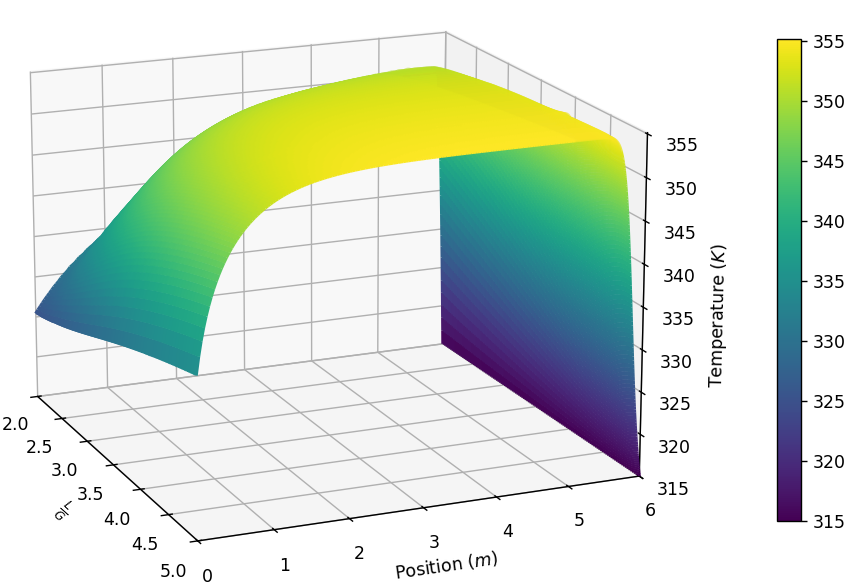
\includegraphics[width=12cm]{figs/Temperature_LG.png}
                \caption{3D surface plot of the temperature profile across the column with varying $\frac{L}{G}$ ratio}\label{fig:3D Temperature}
            \end{figure}
    
            Figure~\ref{fig:3D Temperature} showcases the model’s capabilities using a 3D temperature profile. This figure effectively illustrates the overall behavior of the MEA absorption column model by varying the liquid-to-gas (L/G) ratio, enabling clear visualization of critical phenomena such as the thermodynamic pinch and temperature bulge points within the packed column. This allows clear identification of heat exchange zones like thermodynamic pinch and bulge points, as well as the temperature bulge points where exothermic absorption peaks. To construct this detailed visualization, over 120 individual simulations were executed, each corresponding to specific operating conditions characterized by different L/G ratios. The entire set of simulations was completed in under five minutes, facilitated by the computational efficiency of the numerical solver, with each individual simulation taking approximately three seconds. This rapid simulation time with sufficient accuracy enables extensive parametric studies, providing robust insights into the absorption column’s thermal behavior across a wide operational spectrum.

        \subsection{NCCC Case Study}
        
            We validated the model’s predictive capabilities against the 2017 MEA test campaign data at the NCCC for a one-bed configuration (i.e., without intercoolers) \cite{Morgan2020DevelopmentProcess}. The runs conducted for this campaign are shown in Table \ref{tab:mea-data}.  CO\textsubscript{2} capture percentages closely match those observed in the pilot plant runs, demonstrating that the model provides sufficient accuracy for engineering analyses. This strong agreement between experimental and simulated results underlines the reliability of our open-source framework, establishing a robust foundation for its continued use and refinement in practical applications. Below is an example of the runs that were used to validate the model. Below is an example of the runs that were conducted in a 2017 $\MEA$ test campaign
            
            \begin{table}[htbp]
                \centering
                \small
                \caption{2017 MEA campaign at NCCC}
                \label{tab:mea-data}
                \renewcommand{\arraystretch}{1.2}
                \begin{tabularx}{\textwidth}{|c| *{9}{>{\centering\arraybackslash}X|}}
                \hline
                \textbf{Case} & 
                \makecell{\textbf{Lean Solv.}\\\textbf{Flowrate}\\(kg/h)} &
                \makecell{\textbf{Flue Gas}\\\textbf{Flowrate}\\(kg/h)} &
                \makecell{\textbf{Lean Solv.}\\\textbf{Temp.}\\(°C)} &
                \makecell{\textbf{Flue Gas}\\\textbf{Temp.}\\(°C)} &
                \makecell{\textbf{Absorber}\\\textbf{P}\\(kPa)} &
                \makecell{\textbf{Lean Solv.}\\\textbf{CO\textsubscript{2}}\\\textbf{Loading}} &
                \makecell{\textbf{Lean Solv.}\\\textbf{MEA Mass}\\\textbf{Frac}} &
                \makecell{\textbf{Inlet Flue}\\\textbf{Gas CO\textsubscript{2}}\\\textbf{Mole Frac.}} &
                \makecell{\textbf{$\COtwo$}\\\textbf{Capture}\\\textbf{(\%)}} \\
                \hline
                1A & 8180 & 3000 & 44.1 & 43.4 & 109.4 & 0.24 & 0.30 & 0.082 & 97.5\\
                2A & 7130 & 2690 & 44.9 & 45.2 & 109.5 & 0.25 & 0.31 & 0.087 & 93.4\\
                3A & 3354 & 1500 & 45.6 & 45.2 & 107.9 & 0.24 & 0.31 & 0.073 & 81.1\\
                4A & 3600 & 3000 & 45.6 & 43.4 & 110.2 & 0.19 & 0.31 & 0.076 & 70.6\\
                5A & 3380 & 2750 & 45.5 & 45.7 & 109.8 & 0.20 & 0.31 & 0.107 & 53.9\\
                6A & 3130 & 1750 & 45.1 & 43.4 & 108.2 & 0.31 & 0.30 & 0.106 & 51.7\\
                7A & 4730 & 2255 & 45.1 & 43.5 & 109.2 & 0.23 & 0.30 & 0.109 & 72.5\\
                8A & 3230 & 2240 & 44.8 & 42.8 & 109.2 & 0.24 & 0.31 & 0.107 & 56.3\\
                9A & 3224 & 2245 & 45.9 & 43.4 & 108.8 & 0.14 & 0.31 & 0.108 & 74.2\\
                10A & 7980 & 2492 & 44.8 & 43.1 & 109.0 & 0.32 & 0.30 & 0.109 & 79.9\\
                11A & 3016 & 2761 & 45.8 & 42.9 & 109.6 & 0.16 & 0.30 & 0.096 & 60.5\\
                12A & 4170 & 2920 & 46.4 & 45.1 & 109.7 & 0.14 & 0.30 & 0.092 & 75.4 \\
                13A & 6910 & 2680 & 44.9 & 44.6 & 109.3 & 0.26 & 0.30 & 0.108 & 80.6\\
                14A & 6505 & 2500 & 44.8 & 43.5 & 109.2 & 0.31 & 0.31 & 0.107 & 57.8\\
                15A & 8000 & 2494 & 44.9 & 42.9 & 109.1 & 0.32 & 0.30 & 0.108 & 76.8\\
                1B & 7959 & 2497 & 44.4 & 43.7 & 109.5 & 0.30 & 0.30 & 0.077 & 96.1\\
                2B & 9871 & 2746 & 44.7 & 45.7 & 109.5 & 0.30 & 0.30 & 0.088 & 97.7\\
                3B & 11412 & 2748 & 44.4 & 47.3 & 109.2 & 0.30 & 0.30 & 0.093 & 94.8\\
                1C & 6185 & 1997 & NA & 43.3 & 109.1 & 0.15 & 0.30 & 0.077 & 97.1\\
                2C & 7765 & 2499 & NA & 43.1 & 109.6 & 0.20 & 0.30 & 0.109 & 92.3\\
                3C & 7517 & 2013 & NA & 43.6 & 109.5 & 0.25 & 0.30 & 0.093 & 89.5\\
                4C & 6160 & 1500 & 44.9 & 43.2 & 107.7 & 0.25 & 0.31 & 0.077 & 88.9\\
                5C & 5237 & 1800 & 45.0 & 45.0 & 108.4 & 0.26 & 0.30 & 0.100 & 86.4\\
                6C & 7665 & 2700 & 44.8 & 44.3 & 109.3 & 0.31 & 0.30 & 0.077 & 60.2\\
                7C & 5414 & 1498 & 45.5 & 43.1 & 107.0 & 0.34 & 0.29 & 0.117 & 76.4\\
                1D & 4912 & 2000 & 44.8 & 44.2 & 108.0 & 0.30 & 0.30 & 0.100 & 78.4\\
                2D & 4790 & 1900 & 44.4 & 48.5 & 108.7 & 0.20 & 0.30 & 0.117 & 80.5\\
                3D & 9534 & 2502 & NA & 44.9 & 110.0 & 0.30 & 0.30 & 0.093 & 87.0\\
                4D & 4733 & 1966 & 46.3 & 43.1 & 108.6 & 0.20 & 0.30 & 0.079 & 96.4\\
                \hline
                \end{tabularx}
            \end{table}

        \begin{figure}[ht]
            \centering
            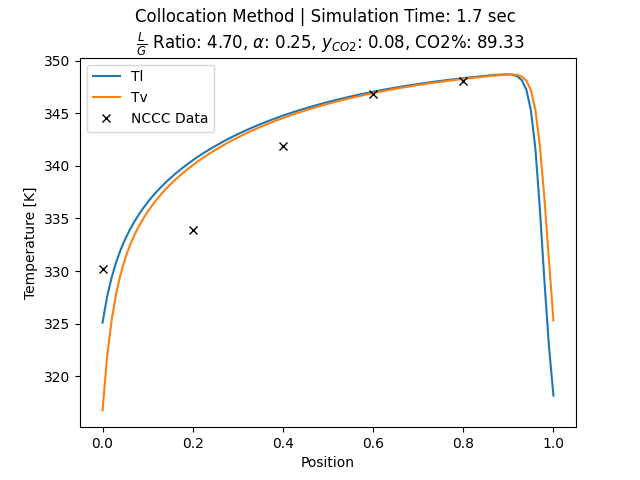
\includegraphics[width=0.9\textwidth]{Figures/Temp_with_data.png}
            \caption{Comparison between modeled temperature profiles and experimental pilot plant column data. The profiles correspond to a liquid-to-gas ratio $\frac{L}{G}$ of 4.70, a CO$_2$ loading $\alpha = 0.25$, and an inlet gas CO$_2$ mole fraction $y_{\mathrm{CO_2}} = 0.08$.}
            \label{fig:temp_profiles}
        \end{figure}
        Case 3C was used as a benchmark run to test the model’s accuracy and performance since it was a simpler case that only requires one bed and no intercoolers included. The temperature data of this row is shown in Table~\ref{tab:3C-temp-profile} 
        \begin{table}[htbp]
            \centering
            \caption{Absorber temperature profile for Case 3C}
            \label{tab:3C-temp-profile}
            \renewcommand{\arraystretch}{1.2}
            \begin{tabular}{|c|c|c|c|c|c|}
                \hline
                \textbf{Relative Column Position} & 0.0 & 0.20 & 0.40 & 0.60 & 0.80 \\
                \hline
                \textbf{Temperature (K)} & 330.2 & 333.0 & 341.9 & 346.9 & 348.1 \\
                \hline
            \end{tabular}
        \end{table}
        The temperature profiles of the solved column are often used to validate since they represent the overall behavior of the column and absorption. The temperature profiles presented in Figure~\ref{fig:temp_profiles} are a critical component for evaluating the physical accuracy and predictive capability of the absorption column model. The plotted curves represent the model-predicted temperature distribution in both the liquid and vapor phases along the column height, overlaid with experimental temperature measurements from a pilot-scale absorber. Matching the overall temperature behavior, particularly the characteristic rise and peak temperature region, provides an essential verification that the energy balances and heat transfer mechanisms are well represented in the model. While perfect agreement with the data is not always expected, a reasonable match to the shape and magnitude of the temperature distribution ensures that the model captures the underlying thermodynamic and mass transfer phenomena governing the $\COtwo$ absorption process. The predicted \% of $\COtwo$ captured by the model also matches very well with the data $\left(89.33\% \:\:\text{vs}\:\:89.50\%\right)$. This validation step strengthens the confidence in the model's ability to be used for further parametric studies, optimization, or scale-up analysis.

       \begin{figure}[ht]
            \centering
            \begin{subfigure}[t]{0.48\textwidth}
                \centering
                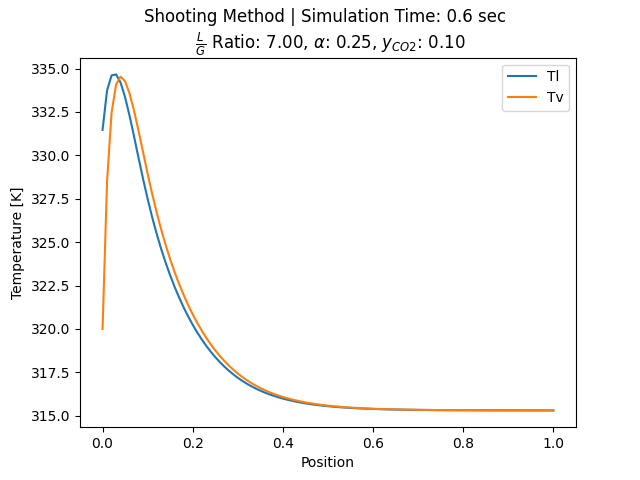
\includegraphics[width=\textwidth]{Figures/shooting.png}
                \caption{Shooting method}
                \label{fig:shooting}
            \end{subfigure}
            \hfill
            \begin{subfigure}[t]{0.48\textwidth}
                \centering
                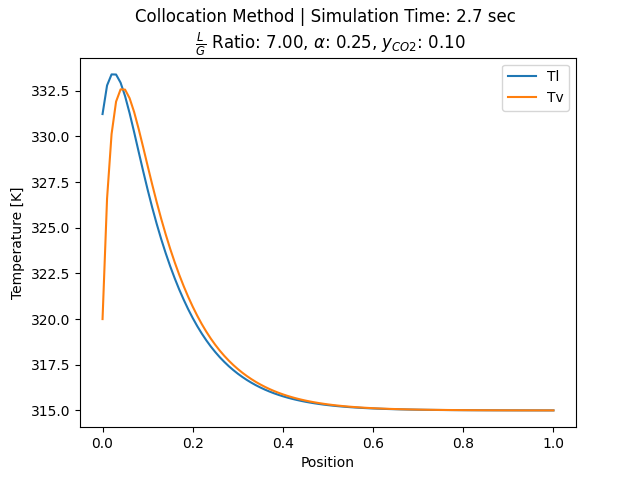
\includegraphics[width=\textwidth]{Figures/collocation.png}
                \caption{Collocation method}
                \label{fig:collocation}
            \end{subfigure}
            \hfill
            \begin{subfigure}[t]{0.48\textwidth}
                \centering
                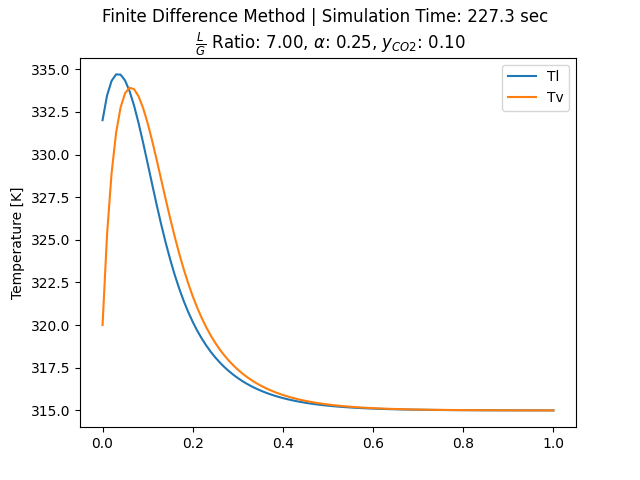
\includegraphics[width=\textwidth]{Figures/finite_difference.png}
                \caption{Finite difference method}
                \label{fig:finite_difference}
            \end{subfigure}
            \caption{Comparison of temperature profiles computed using the shooting method, collocation method, and finite difference method.}
            \label{fig:method_comparison_figures}
        \end{figure}

    \subsection{Simulation Method Comparison}
        Figure~\ref{fig:method_comparison_figures} illustrates the temperature profiles obtained using three numerical methods: shooting, collocation, and finite difference. At higher $L/G$ ratios, the temperature bulge shifts toward the bottom of the column, which generally results in well-conditioned differential equations that the shooting method can solve efficiently. However, when the bulge appears near the top of the column (commonly associated with thermodynamic pinch points) the shooting method becomes unstable or fails to converge due to the stiffness and sensitivity of the coupled ODEs.
        
        The collocation method provides a more robust alternative, particularly well-suited for handling stiff systems. By discretizing the domain and enforcing the equations at multiple collocation points, it is capable of resolving sharp gradients and boundary layer behavior more effectively. The main challenge with this approach is that it typically requires good initial guesses across the entire domain for convergence.
        
        The finite difference method offers yet another solution strategy, and tends to be the most stable across a broad range of operating conditions. As shown in Figure~\ref{fig:finite_difference}, it also produces the smoothest and most physically realistic profiles. However, it is computationally the most demanding. The method requires discretizing all governing equations across many nodes, often involving the simultaneous solution of hundreds of nonlinear algebraic equations. While this can be cumbersome to implement and slower to solve, a properly structured finite difference scheme can serve as a robust backbone for modeling and even process optimization, especially when numerical accuracy is not the top priority.
        
        Each method has trade-offs. The shooting method is fast but limited by stiffness; collocation balances robustness and efficiency but relies on good initial guesses; and finite difference methods are the most stable and smoothest but demand more computational resources and implementation effort. Choose the numerical method based on system stiffness, accuracy needs, and available resources. Table~\ref{tab:method_comparison_table} summarizes these pros and cons as well.
        \begin{table}[ht]
        \centering
        \scriptsize
        \renewcommand{\arraystretch}{1.5}
        \caption{Comparison of numerical methods: Shooting, Collocation, and Finite Difference}
        \label{tab:method_comparison_table}
        \begin{tabular}{|>{\centering\arraybackslash}m{3.5cm}|p{6cm}|p{6cm}|}
            \hline
            \textbf{Method} & \textbf{Pros} & \textbf{Cons} \\
            \hline
            \textbf{Shooting Method} & 
            - Simple and fast implementation \newline
            - Effective for non-stiff systems \newline
            - Leverages standard IVP solvers
            &
            - Struggles with stiff ODE systems \newline
            - Sensitive to initial guesses \newline
            - May fail near thermodynamic pinch \\
            \hline
            \textbf{Collocation Method} &
            - Robust for stiff ODEs \newline
            - Captures sharp gradients effectively \newline
            - Fewer discretization points needed
            &
            - Requires good initial guess across domain \newline
            - More complex implementation \newline
            - Can be slower than shooting method \\
            \hline
            \textbf{Finite Difference Method} &
            - Most numerically stable method \newline
            - Produces smooth, physical profiles \newline
            - Well-suited for stiff and nonlinear models
            &
            - Computationally intensive \newline
            - Requires solving large nonlinear systems \newline
            - More difficult to scale for large grids \\
            \hline
        \end{tabular}
        \end{table}

        If a set of runs were being run on a higher $\frac{L}{G}$ ratio and speed was essential, the shooting method would be the best choice. Each run would finish in less than a second and would converge easily. At a lower $\frac{L}{G}$ ratio, the shooting method struggles to get back the thermodynamic pinch due to the stiffness and non-linearity of the differential equations, and the integrators (like Runge-Kutta) often diverge into infinity. In this case, the finite difference or collocation method would be more suitable. A great strategy to utilize the strength of the methods is to first use the finite difference method to initialize and test the space of the chosen design variable space since this method is the most stable and prone to the least errors. Once the design space is initialized, the results can be used to initialize the guess domain for the collocation method and utilize the speed of its simulations thereafter.


    \subsection{Future Work}    
        Future work includes adding bounds and constraints to the collocation method. It can often struggle if given an initial design variable set that does not correspond well to the predicted solution; the solver will choose infeasible variables such as negative flow rates or critically high temperatures that cause overflow errors. This updated method could be implemented in an object-oriented tool like GEKKO to utilize the quick simulations, stable convergence tools, and the many options the optimizer provides. The drawback to GEKKO, though, is the need to convert the model to be compatible with the GEKKO framework. Further work includes testing novel thermodynamic models using the current fast simulation framework such as ePC-SAFT against other more popular models such as the eNRTL activity coefficient model. Tests can be done to assess simulation time, convergence criteria, and overall performance and best use cases for the various thermodynamic models available. 


    \section{Conclusion}
        This work presents a robust and versatile modeling framework for amine-based absorption columns, offering a fast, accurate, and scalable tool for simulating post-combustion carbon capture (PCC) systems. The integration of detailed mass transfer, thermodynamic, and reaction kinetics components into a modular Python-based platform enables rapid simulation runs, making it ideal for high-throughput parametric studies and design optimization. Validation against pilot data shows the model replicates realistic absorption behavior and thermal profiles across varying conditions, capturing key features such as the thermodynamic pinch and temperature bulge. 3D plots and temperature comparisons confirm the model’s physical consistency across a broad range of operating scenarios, ensuring its reliability for both academic research and industrial design applications.
    
        In addition to model formulation, this study offers a comparative evaluation of three numerical solution methods: shooting, collocation, and finite difference. Each method exhibits unique advantages and trade-offs ranging from the shooting method's simplicity and speed, to collocation’s stiffness-handling robustness, to the finite difference method's superior stability and smoothness. While finite difference methods offer the most consistent results, they come with higher computational costs and complexity. Overall, the collocation method shows to be the best method overall for most circumstances and can even be improved further by adding additional constraints and bounds to its algorithm. These findings underscore the importance of selecting solution techniques based on application-specific priorities such as computational speed, stiffness, and ease of implementation. Ultimately, this work provides not only a validated absorption model but also a practical guide for navigating numerical approaches in PCC simulation, contributing to the broader goal of accelerating the deployment of carbon capture technologies.

    \section*{Code Availability}
        The full Python implementation of the MEA-based absorption column model, including all simulation methods and test data, is available at this
        \href{https://github.com/tannerpolley/MEA_Absorption_Column}{link}

    \section*{Disclaimers}
        The authors declare no financial or commercial conflicts of interest related to this research. One ore more of these authors is a contracted employee with KeyLogic, supporting the National Energy Technology Laboratory (NETL); however, this research was conducted independently and is not associated with their contracted work or responsibilities at NETL.
        \newline
        During the preparation of this work the author(s) used ChatGPT for grammar refinement, restructuring of complex sentences, and generating formatting suggestions for LaTeX.. After using this tool/service, the author(s) reviewed and edited the content as needed and take(s) full responsibility for the content of the publication.

    \clearpage
    \bibliographystyle{model1-num-names}
    \bibliography{mendeley, manual}

    \clearpage
    \appendix
    \vspace{1cm}
    \section{Properties}\label{sec:properties}
        \vspace{1cm}
        \subsection{Thermophysical Properties}
            \vspace{1cm}
            \subsubsection{Henry's Law} 
                To formulate a Henry's Law for the mixture of the liquid solvent, the N2O analogy is used. Below are the equations that help reach the expressions for the solubility of $\COtwo$ in the $\MEA$ from Jiru et al. \cite{Jiru2012}
                \begin{align}
                    H_{\NtwoO,\MEA} &= \left(A_{\NtwoO,\MEA} \times 10^5\right) e^{\frac{-B_{\NtwoO,\MEA}}{T_l}} && \left(\frac{\unit{Pa} \cdot \unit{m}^3}{\unit{mol}} \right)\\
                    H_{\NtwoO,\HtwoO} &= \left(A_{\NtwoO,\HtwoO} \times 10^6\right) e^{\frac{-B_{\NtwoO,\HtwoO}}{T_l}} && \left(\frac{\unit{Pa} \cdot \unit{m}^3}{\unit{mol}} \right)\\
                    H_{\COtwo,\MEA} &= H_{\NtwoO,\MEA} \frac{H_{\COtwo, \HtwoO}}{H_{\NtwoO,\HtwoO}} && \left(\frac{\unit{Pa} \cdot \unit{m}^3}{\unit{mol}} \right)
                \end{align}
                And below is the formulation for the solubility of $\COtwo$ in the $\HtwoO$
                \begin{align}
                    H_{\COtwo, \HtwoO} &= \left(A_{\COtwo, \HtwoO} \times 10^6\right) e^{\frac{-B_{\COtwo, \HtwoO}}{T_l}} && \left(\frac{\unit{Pa} \cdot \unit{m}^3}{\unit{mol}} \right)
                \end{align}
                Next, a deviation is formulated since the solution is not ideal due to the intermolecular forces between the $\MEA$, $\COtwo$, and water. The $Ra$ term is used as the deviation from ideal solubility and uses terms $a_1$, $a_2$, $a_3$, and $b$ coefficients in the functional form.
                \begin{align}
                    R_{a} &= \left(a_1+a_2 \left(T_l-273.15\right)+a_3 \left(T_l-273.15\right)^2+b w_{\HtwoO}\right) w_{\MEA} w_{\HtwoO} \\
                    \sigma &= w_{\MEA} \ln\left(H_{\COtwo,\MEA}\right)+w_{\HtwoO} \ln\left(H_{\COtwo,\HtwoO}\right) \\
                    H_{\COtwo,\text{mix}} &= e^{R_{a} + \sigma} && \left(\frac{\unit{Pa} \cdot \unit{m}^3}{\unit{mol}} \right)
                \end{align}

            \subsubsection{Density}
                The density correlations are below and come from Morgan et al. \cite{Morgan2015}. 
                \begin{align}
                    \shortintertext{\quad\; Liquid Density}
                    V^{\liq}_{\COtwo} &=  a_{\COtwo} + x_{\MEA} x_{\HtwoO} + (b_{\COtwo} + c_{\COtwo} x_{\MEA}) x_{\MEA} x_{\COtwo} \\
                    V^{\liq}_{\MEA} &=  \frac{\text{MW}_{\MEA}}{a_{\MEA} T_l^2 + b_{\MEA} T^{\liq} + c_{\MEA}} + x_{\HtwoO}\left(d_{\MEA} + e_{\MEA}x_{\MEA} \right) \\
                    V^{\liq}_{\HtwoO} &=  \frac{\text{MW}_{\HtwoO}}{a_{\HtwoO} T_l^2 + b_{\HtwoO} T_l + c_{\HtwoO}} \\
                    V^{\liq} &= V^{\liq}_{\COtwo}x_{\COtwo} + V^{\liq}_{\MEA}x_{\MEA} + V^{\liq}_{\HtwoO}x_{\HtwoO} \\
                    \rho ^{\liq}_{mol} &= \frac{1}{V^{\liq}} \\
                    \rho ^{\liq}_{mass} &= \rho ^{\liq}_{mol}\text{MW}^{\liq}_{T} \\
                    \shortintertext{\quad\; Vapor Density}
                    \rho ^{\vap}_{mol} &= \frac{P}{RT_v} \\
                    \rho ^{\vap}_{mass} &= \rho ^{\vap}_{mol}\text{MW}^{\vap}_{T}
                \end{align}

            \subsubsection{Surface Tension} 
            The surface tension correlation is below and come from Morgan et al. \cite{Morgan2015}. 
                \begin{align}
                    \shortintertext{\quad\; First the pure species surface tension expressions are evaluated}
                    \sigma _{\COtwo} &= S_1 r^2+S_2 r+S_3+T_l \left(S_4 r^2+S_5 r+S_6\right) \\
                    \sigma _{\MEA} &= c_{1,\MEA} \left(1-\frac{T_l}{T_{c,\MEA}}\right)^{c_{2,\MEA}+c_{3,\MEA} \frac{T_l}{T_{c,\MEA}}+c_{4,\MEA} \left(\frac{T_l}{T_{c,\MEA}}\right)^2} \\
                    \sigma _{\HtwoO} &= c_{1,\HtwoO} \left(1-\frac{T_l}{T_{c,\HtwoO}}\right)^{c_{2,\HtwoO}+c_{3,\HtwoO} \frac{T_l}{T_{c,\HtwoO}}+c_{4,\HtwoO} \left(\frac{T_l}{T_{c,\HtwoO}}\right)^2} \\
                    \shortintertext{\quad\; The following are added equations to allow for continuous values while the older model only fit for discrete values of r}
                    A &= a+b \alpha+c {\alpha}^2+d w_{\MEA}+e {w_{\MEA}}^2 \\
                    B &= f+g \alpha+h {\alpha}^2+i w_{\MEA}+j {w_{\MEA}}^2 \\
                    \shortintertext{\quad\; The final expression}
                    \sigma _{\text{mix}} &= \sigma_{\HtwoO}+\left(\sigma_{\COtwo}-\sigma_{\HtwoO}\right) A x_{\COtwo}+\left(\sigma_{\MEA}-\sigma_{\HtwoO}\right) B x_{\MEA}
                \end{align}

            \subsubsection{Heat Capacity} 
                A method to calculate heat capacity for solvents originally from Hilliard \cite{Hillard2008}
                \begin{align}
                    C^{\liq}_{p,\MEA} &= 1000 \times \text{\text{MW}}_{\MEA} \sum_{i=0}^{5} {c_{i, \MEA}}^{i} \\
                    C^{\liq}_{p,\HtwoO} &= 1000 \times \text{\text{MW}}_{\HtwoO} \sum_{i=0}^{5} {c_{i, \HtwoO}}^{i} \\
                    C^{\liq}_{p,\COtwo} &= \frac{x_{\MEA} C^{\liq}_{p,\MEA} + x_{\HtwoO} C^{\liq}_{p,\HtwoO}}{x_{\COtwo}} \left( \frac{1}{1 - w_{\COtwo}} - 1\right)
                \end{align}

            \subsubsection{Heat of Vaporization}
                The correlation for heat of vaporization comes from DIPPR \cite{DIPPR2005} with an explicit derivation for the differential of heat of vaporization with respect to temperature for the purpose of evaluating the differential of enthalpy with respect to temperature
                \begin{align}
                    \Delta H_{vap} &= A (1 - T_r)^{B + C T_r + D T_r^2}, \quad \text{where } T_r = \frac{T_l}{T_c} \\
                       \frac{d\Delta H_{vap}}{dT} &= \frac{A \cdot \left( \frac{T_c - T}{T_c} \right)^{\frac{BT_c^2 + CTT_c + DT^2}{T_c^2}} \cdot \left[ BT_c^2 + CTT_c + DT^2 + (T - T_c)(CT_c + 2DT) \cdot \ln\left( \frac{T_c - T}{T_c} \right) \right]}{T_c^2(T - T_c)}
                \end{align}

            \subsubsection{Enthalpy}
                The original correlations come from Akula \cite{Akula2023AppendixAkula} but they were revised to the current versions for this model
                \begin{align}
                    \shortintertext{\quad\; Pure Species Enthalpies}
                    H^{\liq}_{\COtwo} &= H_{\text{CO}_2}^V - RT^2 \left( \frac{\partial \ln H_{\text{CO}_2, \text{H}_2\text{O}}}{\partial T} \right) + \Delta H_{abs} \\
                    H^{\liq}_{\COtwo} &= H_{\text{CO}_2}^V - R \left( -b_{\text{CO}_2, \text{H}_2\text{O}} + c_{\text{CO}_2, \text{H}_2\text{O}} T + d_{\text{CO}_2, \text{H}_2\text{O}} T^2 \right) + \Delta H_{abs} \\
                    H^{\liq}_{\MEA} &= \int_{T_{ref}}^{T} C_{p,\MEA} dT - \Delta H_{vap, \MEA} \\
                    H^{\liq}_{\HtwoO} &= \int_{T_{ref}}^{T} C_{p,\HtwoO} dT - \Delta H_{vap, \HtwoO} \\
                    \shortintertext{\quad\; Total enthalpy for liquid phase}
                    H^{\liq}_{T} &= \sum_{i} x_iH^{\liq}_{i} \\
                    \shortintertext{\quad\; Liquid enthalpy differential with respect to temperature for temperature based energy-balance derivation}
                    \frac{H^{\liq}_{T}}{dT} &= -R\left(c_{\text{CO}_2, \text{H}_2\text{O}}  + 2d_{\text{CO}_2, \text{H}_2\text{O}} T \right) + C^{\liq}_{p, \MEA} + \frac{d\Delta H_{vap, \MEA}}{dT} +  C^{\liq}_{p, \HtwoO}+ \frac{d\Delta H_{vap, \HtwoO}}{dT}
                \end{align}

            \subsubsection{Thermal Conductivity}
                \begin{align}
                    k^{t}_{i} = \frac{A_i T^{B_i}}{1 + \frac{C_i}{T} + \frac{D_i}{T^2}}
                \end{align}

        \newpage
        \subsection{Transport Properties}
            \subsubsection{Viscosity} \cite{Morgan2015}
                \textbf{Liquid Viscosity}
                \begin{align}
                    \mu ^{\liq}_{\HtwoO} &= A \times 10^\frac{B\left(293.15 - T_l - C\left(T_l - 293.15\right)^2\right)}{T_l - D} \\
                    R &= \ln\left(mu^{\vap}_{\COtwo}\right) y_{\COtwo}+\ln\left(mu^{\vap}_{\HtwoO}\right) y_{\HtwoO}+\ln\left(mu^{\vap}_{N_2}\right) y_{N_2}+\ln\left(mu^{\vap}_{O_2}\right) y_{O_2} \\
                    \mu ^{\liq}_{\text{mix}} &= \mu ^{\liq}_{\HtwoO} \times e^{R}
                \end{align}
                \vspace{.5cm}
                \textbf{Vapor Viscosity}
                \begin{align}
                    \mu ^{\vap}_{\COtwo} &= \frac{2.148 \times 10^{-6} \ T_v^{0.46}}{1+\frac{290}{T_v}} \\
                    \mu ^{\vap}_{\HtwoO} &= 1.7096\times 10^{-8} \ T_v^{1.1146} \\
                    \mu ^{\vap}_{N_2} &= \frac{6.5592\times 10^{-7} \ T_v^{0.6081}}{1+\frac{54.714}{T_v}} \\
                    \mu ^{\vap}_{O_2} &= \frac{5.5462\times 10^{-8} \ T_v^{0.8825}}{1+\frac{73.316}{T_v}} \\
                    R &= \ln\left(\mu^{\vap}_{\COtwo}\right) y_{\COtwo}+\ln\left(\mu^{\vap}_{\HtwoO}\right) y_{\HtwoO}+\ln\left(\mu^{\vap}_{N_2}\right) y_{N_2}+\ln\left(\mu^{\vap}_{O_2}\right) y_{O_2} \\
                    \theta_{ij} &= \frac{1 + 2\,\sqrt{\frac{\mu^{\vap}_{i}}{\mu^{\vap}_{j}}}\left(\frac{\text{MW}^{\vap}_{j}}{\text{MW}^{\vap}_{i}}\right)^{0.25} + \frac{\mu^{\vap}_{i}}{\mu^{\vap}_{j}}\left(\frac{\text{MW}^{\vap}_{j}}{\text{MW}^{\vap}_{i}}\right)^{0.5}}{\sqrt{8 + 8\,\frac{\text{MW}^{\vap}_{i}}{\text{MW}^{\vap}_{j}}}} \\
                    \theta_{ji} &= \frac{\mu ^{\vap}_{j}}{mu ^{\vap}_{i}}\frac{\text{MW}^{\vap}_{i}}{\text{MW}^{\vap}_{j}}\theta_{ij}  \\
                    \theta_{ij} &= 1 \quad\Longrightarrow\quad \text{if } i = j \\
                    \mu^{\vap}_{\text{mix}} &= \sum_{i=1}^{N} \frac{y_i \,\mu^{\vap}_{i}}{\sum_{j=1}^{N} y_j \,\theta_{i,j}}
                \end{align}

            \subsubsection{Diffusivity}
                \textbf{Liquid Diffusivity}
                \begin{align}
                    C^{\liq}_{\MEA,\text{true}} &= C^{\liq}_{\MEA} \times 10^{-3} \\
                    D^{\liq}_{ \COtwo} &= \left(a + b C^{\liq}_{\MEA,\text{true}} + c {C^{\liq}_{\MEA,\text{true}}}^2\right) e^{\frac{d + e C^{\liq}_{\MEA,\text{true}}}{T_l}} \\
                    D^{\liq}_{ \MEA} &= e^{a + \frac{b}{T_l} + c C^{\liq}_{\MEA}} \\
                    D^{\liq}_{ \text{ion}} &= e^{a + \frac{b}{T_l} + c \log{\mu ^{\liq}_{ \text{mix}}}}
                \end{align}
                \vspace{.5cm}
                \textbf{Vapor Diffusivity}
                \begin{align}
                    D_{i j} &= 1.013 \times 10^{-2} T_V^{1.75} \frac{\sqrt{\left(\text{MW}^{\vap}_{i}+\text{MW}^{\vap}_{j}\right) / \text{MW}^{\vap}_{i} \text{MW}^{\vap}_{j}}}{P\left(\sqrt[3]{V_{D i}}+\sqrt[3]{V_{D j}}\right)^2} \\
                    D^{\vap}_{ i} &= \frac{1-y_i}{\sum_{\substack{j=1 \\ j \neq i}}^n \frac{y_j}{D_{i j}}}
                \end{align}

        \newpage
        \subsection{Constants}
        
\begin{longtable}{lll}
\label{tab:constants_table}\\
\caption{Constants used in the model} \\
\hline
\textbf{Constant}      & \textbf{Variable} & \textbf{Value} \\
\hline
\endhead
%
Column Diameter         & $D$               & 0.64           \\
Column Height           & $H$               & 6              \\
Gas Constant            & $R$               & 8.314463       \\
Gravitational Constant  & $g$               & 9.806          \\
Specific Packing        & $a_p$             & 250            \\
Void Packing            & $\epsilon$        & 0.97           \\
Liquid Packing          & $C_l$             & 0.203          \\
Vapor Packing           & $C_v$             & 0.35           \\
\hline
\end{longtable}

        \newpage
        \subsection{Parameters}

\begin{longtable}{lllll}
% \label{tab:parameters_table}\\
\caption{Parameters used in the model} \\
\hline
\textbf{Parameter Type} & \textbf{Phase} & \textbf{Species}    & \textbf{Variable} & \textbf{Value} \\ \hline
\endhead
%
Henry's Law               & Liquid         & $\ce{N2O},\ce{MEA}$ & $a$               & 2.4480E+05     \\
Henry's Law               & Liquid         & $\ce{N2O},\ce{MEA}$ & $b$               & 1348           \\
Henry's Law               & Liquid         & $\ce{CO2},\ce{H2O}$ & $a$               & 3.5200E+06     \\
Henry's Law               & Liquid         & $\ce{CO2},\ce{H2O}$ & $b$               & 2113           \\
Henry's Law               & Liquid         & $\ce{N2O},\ce{H2O}$ & $a$               & 8.4490E+06     \\
Henry's Law               & Liquid         & $\ce{N2O},\ce{H2O}$ & $b$               & 2283           \\
Henry's Law               & Liquid         & mixture             & $a_1$             & -2.0761        \\
Henry's Law               & Liquid         & mixture             & $a_2$             & 3.7322E-02     \\
Henry's Law               & Liquid         & mixture             & $a_3$             & -3.2721E-04    \\
Henry's Law               & Liquid         & mixture             & $b$               & -0.1111        \\
Density                   & Liquid         & $\ce{CO2}$          & $a$               & -10.5792       \\
Density                   & Liquid         & $\ce{CO2}$          & $b$               & 192.0126       \\
Density                   & Liquid         & $\ce{CO2}$          & $c$               & -695.3849      \\
Density                   & Liquid         & $\ce{MEA}$          & $a$               & -5.3516E-07    \\
Density                   & Liquid         & $\ce{MEA}$          & $b$               & -4.5142E-04    \\
Density                   & Liquid         & $\ce{MEA}$          & $c$               & 1.1945         \\
Density                   & Liquid         & $\ce{MEA}$          & $d$               & -2.0205        \\
Density                   & Liquid         & $\ce{MEA}$          & $e$               & 3.1507         \\
Density                   & Liquid         & $\ce{H2O}$          & $a$               & -3.2484E-06    \\
Density                   & Liquid         & $\ce{H2O}$          & $b$               & 1.6500E-03     \\
Density                   & Liquid         & $\ce{H2O}$          & $c$               & 0.793          \\
Surface Tension           & Liquid         & mixture             & $S_1$             & -5.8993E-03    \\
Surface Tension           & Liquid         & mixture             & $S_2$             & 1.7502E-03     \\
Surface Tension           & Liquid         & mixture             & $S_3$             & 0.1297         \\
Surface Tension           & Liquid         & mixture             & $S_4$             & 1.2644E-05     \\
Surface Tension           & Liquid         & mixture             & $S_5$             & -5.7395E-06    \\
Surface Tension           & Liquid         & mixture             & $S_6$             & -1.8969E-04    \\
Surface Tension           & Liquid         & $\ce{MEA}$          & $c_1$             & 9.9450E-02     \\
Surface Tension           & Liquid         & $\ce{MEA}$          & $c_2$             & 1.067          \\
Surface Tension           & Liquid         & $\ce{MEA}$          & $c_3$             & 0              \\
Surface Tension           & Liquid         & $\ce{MEA}$          & $c_4$             & 0              \\
Surface Tension           & Liquid         & $\ce{MEA}$          & $T_c$             & 614.45         \\
Surface Tension           & Liquid         & $\ce{H2O}$          & $c_1$             & 0.1855         \\
Surface Tension           & Liquid         & $\ce{H2O}$          & $c_2$             & 2.717          \\
Surface Tension           & Liquid         & $\ce{H2O}$          & $c_3$             & -3.554         \\
Surface Tension           & Liquid         & $\ce{H2O}$          & $c_4$             & 2.047          \\
Surface Tension           & Liquid         & $\ce{H2O}$          & $T_c$             & 647.13         \\
Surface Tension           & Liquid         & mixture             & $a$               & 1070.6567      \\
Surface Tension           & Liquid         & mixture             & $b$               & -2578.7813     \\
Surface Tension           & Liquid         & mixture             & $c$               & 3399.2411      \\
Surface Tension           & Liquid         & mixture             & $d$               & -2352.4741     \\
Surface Tension           & Liquid         & mixture             & $e$               & 2960.2475      \\
Surface Tension           & Liquid         & mixture             & $f$               & 3.0668         \\
Surface Tension           & Liquid         & mixture             & $g$               & -1.7944        \\
Surface Tension           & Liquid         & mixture             & $h$               & -7.2124        \\
Surface Tension           & Liquid         & mixture             & $i$               & 2.975          \\
Surface Tension           & Liquid         & mixture             & $j$               & -10.5739       \\
Heat Capacity             & Liquid         & $\ce{CO2}$          & $a$               & 2.7637E+05     \\
Heat Capacity             & Liquid         & $\ce{CO2}$          & $b$               & -2090.1        \\
Heat Capacity             & Liquid         & $\ce{CO2}$          & $c$               & 8.125          \\
Heat Capacity             & Liquid         & $\ce{CO2}$          & $d$               & -1.4116E-02    \\
Heat Capacity             & Liquid         & $\ce{CO2}$          & $e$               & 9.3701E-06     \\
Heat Capacity             & Liquid         & $\ce{MEA}$          & $a$               & 2.6161         \\
Heat Capacity             & Liquid         & $\ce{MEA}$          & $b$               & 3.7060E-03     \\
Heat Capacity             & Liquid         & $\ce{MEA}$          & $c$               & 3.7870E-06     \\
Heat Capacity             & Liquid         & $\ce{MEA}$          & $d$               & 0              \\
Heat Capacity             & Liquid         & $\ce{MEA}$          & $e$               & 0              \\
Heat Capacity             & Liquid         & $\ce{H2O}$          & $a$               & 4.2107         \\
Heat Capacity             & Liquid         & $\ce{H2O}$          & $b$               & -1.6960E-03    \\
Heat Capacity             & Liquid         & $\ce{H2O}$          & $c$               & 2.5680E-05     \\
Heat Capacity             & Liquid         & $\ce{H2O}$          & $d$               & -1.0950E-07    \\
Heat Capacity             & Liquid         & $\ce{H2O}$          & $e$               & 3.0380E-10     \\
Heat of Vaporization      & Liquid         & $\ce{CO2}$          & $a$               & 2.1730E+07     \\
Heat of Vaporization      & Liquid         & $\ce{CO2}$          & $b$               & 0.382          \\
Heat of Vaporization      & Liquid         & $\ce{CO2}$          & $c$               & -0.4339        \\
Heat of Vaporization      & Liquid         & $\ce{CO2}$          & $d$               & 0.4221         \\
Heat of Vaporization      & Liquid         & $\ce{CO2}$          & $T_c$             & 304.21         \\
Heat of Vaporization      & Liquid         & $\ce{MEA}$          & $a$               & 8.2393E+07     \\
Heat of Vaporization      & Liquid         & $\ce{MEA}$          & $b$               & 0.5905         \\
Heat of Vaporization      & Liquid         & $\ce{MEA}$          & $c$               & -0.436         \\
Heat of Vaporization      & Liquid         & $\ce{MEA}$          & $d$               & 0.3784         \\
Heat of Vaporization      & Liquid         & $\ce{MEA}$          & $T_c$             & 678.2          \\
Heat of Vaporization      & Liquid         & $\ce{H2O}$          & $a$               & 5.6600E+07     \\
Heat of Vaporization      & Liquid         & $\ce{H2O}$          & $b$               & 0.612          \\
Heat of Vaporization      & Liquid         & $\ce{H2O}$          & $c$               & -0.6257        \\
Heat of Vaporization      & Liquid         & $\ce{H2O}$          & $d$               & 0.3988         \\
Heat of Vaporization      & Liquid         & $\ce{H2O}$          & $T_c$             & 647.096        \\
Heat of Absorption        & Liquid         & $\ce{CO2}$          & $\Delta H_{abs}$  & -8.4000E+04    \\
Heat Capacity             & Vapor          & $\ce{CO2}$          & $c_1$             & 5.457          \\
Heat Capacity             & Vapor          & $\ce{CO2}$          & $c_2$             & 1.0450E-03     \\
Heat Capacity             & Vapor          & $\ce{CO2}$          & $c_3$             & -1.1570E+05    \\
Heat Capacity             & Vapor          & $\ce{H2O}$          & $c_1$             & 3.47           \\
Heat Capacity             & Vapor          & $\ce{H2O}$          & $c_2$             & 1.4500E-03     \\
Heat Capacity             & Vapor          & $\ce{H2O}$          & $c_3$             & 1.2100E+04     \\
Heat Capacity             & Vapor          & $\ce{N2}$           & $c_1$             & 3.28           \\
Heat Capacity             & Vapor          & $\ce{N2}$           & $c_2$             & 5.9300E-04     \\
Heat Capacity             & Vapor          & $\ce{N2}$           & $c_3$             & 4000           \\
Heat Capacity             & Vapor          & $\ce{O2}$           & $c_1$             & 3.639          \\
Heat Capacity             & Vapor          & $\ce{O2}$           & $c_2$             & 5.0600E-04     \\
Heat Capacity             & Vapor          & $\ce{O2}$           & $c_3$             & -2.2700E+04    \\
Thermal Conductivity      & Vapor          & $\ce{CO2}$          & $a$               & 3.69           \\
Thermal Conductivity      & Vapor          & $\ce{CO2}$          & $b$               & -0.3838        \\
Thermal Conductivity      & Vapor          & $\ce{CO2}$          & $c$               & 964            \\
Thermal Conductivity      & Vapor          & $\ce{CO2}$          & $d$               & 1.8600E+06     \\
Thermal Conductivity      & Vapor          & $\ce{H2O}$          & $a$               & 6.2040E-06     \\
Thermal Conductivity      & Vapor          & $\ce{H2O}$          & $b$               & 1.3973         \\
Thermal Conductivity      & Vapor          & $\ce{H2O}$          & $c$               & 0              \\
Thermal Conductivity      & Vapor          & $\ce{H2O}$          & $d$               & 0              \\
Thermal Conductivity      & Vapor          & $\ce{N2}$           & $a$               & 3.3100E-04     \\
Thermal Conductivity      & Vapor          & $\ce{N2}$           & $b$               & 0.7722         \\
Thermal Conductivity      & Vapor          & $\ce{N2}$           & $c$               & 16.323         \\
Thermal Conductivity      & Vapor          & $\ce{N2}$           & $d$               & 373.72         \\
Thermal Conductivity      & Vapor          & $\ce{O2}$           & $a$               & 4.5000E-04     \\
Thermal Conductivity      & Vapor          & $\ce{O2}$           & $b$               & 0.7456         \\
Thermal Conductivity      & Vapor          & $\ce{O2}$           & $c$               & 56.699         \\
Thermal Conductivity      & Vapor          & $\ce{O2}$           & $d$               & 0              \\
Vapor Pressure            & Liquid         & $\ce{H2O}$          & $a$               & 72.55          \\
Vapor Pressure            & Liquid         & $\ce{H2O}$          & $b$               & -7206.7        \\
Vapor Pressure            & Liquid         & $\ce{H2O}$          & $c$               & -7.1385        \\
Vapor Pressure            & Liquid         & $\ce{H2O}$          & $d$               & 4.0500E-06     \\
Viscosity                 & Liquid         & $\ce{H2O}$          & $a$               & 1.0020E-03     \\
Viscosity                 & Liquid         & $\ce{H2O}$          & $b$               & 1.3272         \\
Viscosity                 & Liquid         & $\ce{H2O}$          & $c$               & 1.0530E-03     \\
Viscosity                 & Liquid         & $\ce{H2O}$          & $d$               & 168.15         \\
Viscosity                 & Liquid         & mixture             & $a$               & -8.5404E-02    \\
Viscosity                 & Liquid         & mixture             & $b$               & 2.7291         \\
Viscosity                 & Liquid         & mixture             & $c$               & 35.1159        \\
Viscosity                 & Liquid         & mixture             & $d$               & 1805.5276      \\
Viscosity                 & Liquid         & mixture             & $e$               & 7.1603E-03     \\
Viscosity                 & Liquid         & mixture             & $f$               & 1.0649E-02     \\
Viscosity                 & Liquid         & mixture             & $g$               & -8.5404E-02    \\
Viscosity                 & Vapor          & $\ce{CO2}$          & $a$               & 2.1480E-06     \\
Viscosity                 & Vapor          & $\ce{CO2}$          & $b$               & 0.46           \\
Viscosity                 & Vapor          & $\ce{CO2}$          & $c$               & 290            \\
Viscosity                 & Vapor          & $\ce{H2O}$          & $a$               & 1.7096E-08     \\
Viscosity                 & Vapor          & $\ce{H2O}$          & $b$               & 1.1146         \\
Viscosity                 & Vapor          & $\ce{N2}$           & $a$               & 1.7810E-05     \\
Viscosity                 & Vapor          & $\ce{N2}$           & $b$               & 300.55         \\
Viscosity                 & Vapor          & $\ce{N2}$           & $c$               & 111            \\
Viscosity                 & Vapor          & $\ce{O2}$           & $a$               & 2.0180E-05     \\
Viscosity                 & Vapor          & $\ce{O2}$           & $b$               & 292.25         \\
Viscosity                 & Vapor          & $\ce{O2}$           & $c$               & 127            \\
Diffusivity               & Liquid         & $\ce{CO2}$          & $a$               & 2.3500E-06     \\
Diffusivity               & Liquid         & $\ce{CO2}$          & $b$               & 2.9837E-08     \\
Diffusivity               & Liquid         & $\ce{CO2}$          & $c$               & -9.7078E-09    \\
Diffusivity               & Liquid         & $\ce{CO2}$          & $d$               & -2119          \\
Diffusivity               & Liquid         & $\ce{CO2}$          & $e$               & -20.132        \\
Diffusivity               & Liquid         & $\ce{MEA}$          & $a$               & -13.275        \\
Diffusivity               & Liquid         & $\ce{MEA}$          & $b$               & -2198.3        \\
Diffusivity               & Liquid         & $\ce{MEA}$          & $c$               & -7.8142E-05    \\
Diffusivity               & Liquid         & $\ce{MEA}$          & $a$               & -22.64         \\
Diffusivity               & Liquid         & $\ce{MEA}$          & $b$               & -1000          \\
Diffusivity               & Liquid         & $\ce{MEA}$          & $c$               & -0.7           \\
Diffusivity               & Vapor          & $\ce{CO2}$          & $a$               & 26.7           \\
Diffusivity               & Vapor          & $\ce{H2O}$          & $b$               & 13.1           \\
Diffusivity               & Vapor          & $\ce{N2}$           & $c$               & 18.5           \\
Diffusivity               & Vapor          & $\ce{O2}$           & $d$               & 16.3           \\
Interfacial Area          &                &                     & $A_1$             & 1.4391         \\
Interfacial Area          &                &                     & $A_2$             & 0.12           \\
Liquid Hold Up            &                &                     & $A$               & 11.4474        \\
Liquid Hold Up            &                &                     & $B$               & 0.6471         \\
Liquid Hold Up            &                &                     & $\alpha$          & 3.186          \\
Carbamate Rate Constant   &                &                     & $a$               & 233.4          \\
Carbamate Rate Constant   &                &                     & $b$               & -3410          \\
Carbamate Rate Constant   &                &                     & $c$               & -36.8          \\
Carbamate Rate Constant   &                &                     & $d$               & 0              \\
Bicarbonate Rate Constant &                &                     & $a$               & 176.72         \\
Bicarbonate Rate Constant &                &                     & $b$               & -2909          \\
Bicarbonate Rate Constant &                &                     & $c$               & -28.46         \\
Bicarbonate Rate Constant &                &                     & $d$               & 0              \\
\hline
\end{longtable}

\newpage
\subsection{Code Snippet of Model}

\begin{lstlisting}[language=Python, caption={Absorption Column Function}, label={lst:abs_column}]
import numpy as np
from MEA_Absorption_Column.Parameters import MWs_l
from MEA_Absorption_Column.Properties.Thermophysical_Properties import (density, surface_tension, heat_capacity, thermal_conductivity, henrys_law, enthalpy, vapor_pressure)
from MEA_Absorption_Column.Properties.Transport_Properties import viscosity, diffusivity
from MEA_Absorption_Column.Thermodynamics.Fugacity import fugacity
from MEA_Absorption_Column.Thermodynamics.Chemical_Equilibrium import chemical_equilibrium
from MEA_Absorption_Column.Transport.Hydraulic_Variables_Correlations import (velocity, holdup, interfacial_area, flooding_fraction)
from MEA_Absorption_Column.Transport.Transfer_Coefficients import mass_transfer_coeff, heat_transfer_coeff
from MEA_Absorption_Column.Transport.Pressure_Drop import pressure_drop
from MEA_Absorption_Column.Transport.Enhancement_Factor import enhancement_factor
from MEA_Absorption_Column.Transport.Flux import molar_flux, enthalpy_flux
from MEA_Absorption_Column.misc.Get_Temperature_Enthalpy import get_liquid_temperature, get_vapor_temperature
from MEA_Absorption_Column.misc.special_functions import f_dHl_dT


def abs_column(zi, Y_scaled, parameters, run_type='simulating', column_names=False):
    # Unpack System Parameters
    scales, eq_scales, const_flow, H, A, packing = parameters
    Fl_MEA, Fv_N2, Fv_O2 = const_flow

    # Define System Variables
    Y = np.array(Y_scaled) * np.array(scales)

    Fl_CO2, Fl_H2O, Fv_CO2, Fv_H2O, Hlf, Hvf, P = Y

    Fl_T = Fl_CO2 + Fl_MEA + Fl_H2O
    Fv_T = Fv_CO2 + Fv_H2O + Fv_N2 + Fv_O2

    Fl = [Fl_CO2, Fl_MEA, Fl_H2O]
    Fv = [Fv_CO2, Fv_H2O, Fv_N2, Fv_O2]

    x = [Fl[i] / Fl_T for i in range(len(Fl))]
    y = [Fv[i] / Fv_T for i in range(len(Fv))]

    Hl = Hlf / Fl_T
    Hv = Hvf / Fv_T

    Tl = get_liquid_temperature(x, Hl)
    Tv = get_vapor_temperature(y, Hv)

    w = [MWs_l[i] * x[i] / sum([MWs_l[j] * x[j] for j in range(len(Fl))]) for i in range(len(Fl))]

    alpha = x[0] / x[1]
    w_MEA = w[1]
    w_H2O = w[2]

    # Properties

    # Thermophysical Properties

    # Henry's Law
    H_CO2_mix = henrys_law(Tl, x)

    # Density
    rho_mol_l, rho_mass_l, volume = density(Tl, x, P, phase='liquid')
    rho_mol_v, rho_mass_v = density(Tv, y, P, phase='vapor')

    # Surface Tension
    sigma = surface_tension(Tl, x, w_MEA, w_H2O)

    # Heat Capacity
    Cpl, Cpl_T = heat_capacity(Tl, x, phase='liquid')
    Cpv, Cpv_T = heat_capacity(Tv, y, phase='vapor')

    # Enthalpy
    Hl, Hl_T = enthalpy(Tl, x, phase='liquid') # J/mol
    Hl_CO2, Hl_MEA, Hl_H2O = Hl
    Hv, Hv_T = enthalpy(Tv, y, phase='vapor')  # J/mol
    Hv_CO2, Hv_H2O, Hv_N2, Hv_O2 = Hv

    # Vapor Pressure
    P_sat_H2O = vapor_pressure(Tl)

    # Transport Properties

    # Viscosity
    mul_mix, mul_H2O = viscosity(Tl, x, w_MEA, w_H2O, phase='liquid')
    muv_mix, muv = viscosity(Tv, y, w_MEA, w_H2O, phase='vapor')

    # Diffusivity
    Dl_CO2, Dl_MEA, Dl_ion = diffusivity(Tl, x, P, mul_mix, rho_mol_l, phase='liquid')
    Dv_CO2, Dv_H2O, Dv_N2, Dv_O2, Dv_T = diffusivity(Tv, y, P, mul_mix, rho_mol_l, phase='vapor')

    # Thermal Conductivity
    kt_vap = thermal_conductivity(Tv, y, muv)

    # Thermodynamics

    # Chemical Equilibrium
    Cl_true, x_true = chemical_equilibrium(Fl.copy(), Tl)

    Cl = [x[i] * rho_mol_l for i in range(len(x))]
    Cv = [y[i] * rho_mol_v for i in range(len(y))]

    Cl_true = [x_true[i] * rho_mol_l for i in range(len(x_true))]

    # Vapor-Liquid Equilibrium
    fl_CO2, fv_CO2, fl_H2O, fv_H2O, CO2, H2O = fugacity(x, y, x_true, Cl_true, Tl, Tv, alpha, H_CO2_mix, P, P_sat_H2O)

    # Transport

    # Hydraulic Variables

    # Velocity
    ul, uv = velocity(rho_mol_l, rho_mol_v, A, Fl_T, Fv_T)

    # Interfacial Area
    a_e, a_eA = interfacial_area(rho_mass_l, sigma, ul, A, packing)

    # Holdup
    h_L, h_V = holdup(ul, mul_mix, rho_mass_l, packing)

    # Flooding Fraction
    fl_frac = flooding_fraction(rho_mass_l, rho_mass_v, mul_mix, mul_H2O, Fl_T, Fv_T, uv, packing)

    # Transfer Coefficients

    # Mass Transfer Coefficients
    kl_CO2, kv_CO2, kv_H2O, kv_T, const = mass_transfer_coeff(h_L, h_V, rho_mass_v, muv_mix, Dl_CO2, Dv_CO2, Dv_H2O,
                                                              Dv_T, A, Tv, ul, uv, packing)

    # Heat Transfer Coefficient
    UT = heat_transfer_coeff(P, kv_CO2, kt_vap, Cpv_T, rho_mol_v, Dv_CO2, a_eA)  # J/(s*K*m) or W/(K*m)

    # Pressure Drop
    delta_P_H = pressure_drop(h_L, rho_mass_l, rho_mass_v, mul_mix, muv_mix, A, ul, uv, packing)

    # Enhancement Factor
    E, Psi, Psi_H, enhance_factor = enhancement_factor(Tl, Cl_true, y[0], P, H_CO2_mix, kl_CO2, kv_CO2,
                                                       Dl_CO2, Dl_MEA, Dl_ion, E_type='implicit')

    # Flux

    # Molar Flux
    Nv_CO2, Nv_H2O, Nl_CO2, Nl_H2O = molar_flux(fl_CO2, fv_CO2, fl_H2O, fv_H2O, kv_CO2, kv_H2O, a_eA, Psi_H)

    # Enthalpy Flux
    Hv_flux, Hl_flux, qv, ql, Hv_trn, Hl_trn, Hv_CO2_trn, Hv_H2O_trn, Hl_CO2_trn, Hl_H2O_trn = enthalpy_flux(Nl_CO2, Hl_CO2, Nl_H2O, Hl_H2O, Nv_CO2, Hv_CO2, Nv_H2O, Hv_H2O, UT, a_eA, Tv, Tl)

    # Balance Equations

    # Mass Balance
    dFl_CO2_dz = -Nl_CO2 + 1e-10  # mol/(s*m)
    dFl_H2O_dz = -Nl_H2O + 1e-10  # mol/(s*m)

    dFv_CO2_dz = Nv_CO2 + 1e-10  # mol/(s*m)
    dFv_H2O_dz = Nv_H2O + 1e-10  # mol/(s*m)

    # Energy Balance
    dHlf_dz = Hl_flux + 1e-10
    dHvf_dz = Hv_flux + 1e-10

    dHl_dT = f_dHl_dT(Tl, x)
    dHv_dT = Cpv_T

    dTl_dz = H*(Hl_flux + Hl_T*(Nl_CO2 + Nl_H2O))/(Fl_T*dHl_dT) # K/m
    dTv_dz = H*(Hv_flux - Hv_T*(Nv_CO2 + Nv_H2O))/(Fv_T*dHv_dT)

    # Momentum Balance
    dP_dz = 0  # Pa/m

    # Run Output

    if run_type == 'simulating':
        # Combine Differentials and Scale
        diffeqs = np.array([dFl_CO2_dz, dFl_H2O_dz, dFv_CO2_dz, dFv_H2O_dz, dHlf_dz, dHvf_dz, dP_dz])
        # eq_scales = np.array([1, 1, 50, 50, 200000, 200000, P])
        diffeqs_scaled = diffeqs / scales * H
        return diffeqs_scaled

    elif run_type == 'saving':
        Fl_true = [Cl_true[i] * ul * A for i in range(len(Cl_true))]

        Fl_CO2, Fl_MEA, Fl_H2O = Fl
        Fl_CO2_true, Fl_MEA_true, Fl_H2O_true, Fl_MEAH_true, Fl_MEACOO_true, Fl_HCO3_true = Fl_true
        Fv_CO2, Fv_H2O, Fv_N2, Fv_O2 = Fv
        Cl_CO2, Cl_MEA, Cl_H2O = Cl
        Cl_CO2_true, Cl_MEA_true, Cl_H2O_true, Cl_MEAH_true, Cl_MEACOO_true, Cl_HCO3_true = Cl_true
        x_CO2, x_MEA, x_H2O = x
        x_CO2_true, x_MEA_true, x_H2O_true, x_MEAH_true, x_MEACOO_true, x_HCO3_true = x_true
        y_CO2, y_H2O, y_N2, y_O2 = y
        Cv_CO2, Cv_H2O, Cv_N2, Cv_O2 = Cv
        DF_CO2, H_CO2_mix = CO2
        DF_H2O, Psat_H2O = H2O
        k2, Cl_MEA_true, Dl_CO2, kl_CO2, Ha, E, Psi_H, Psi = enhance_factor
        Cpl_CO2, Cpl_MEA, Cpl_H2O = Cpl
        Cpv_CO2, Cpv_H2O, Cpv_N2, Cpv_O2 = Cpv
        V_l, V_CO2, V_MEA, V_H2O = volume
        Hl_CO2 = Hl_CO2 + 1e-5
        Clp, Cvp, eps, a_p, A, Lp, d_h = const
        muv_CO2, muv_H2O, muv_N2, muv_O2 = muv

        output_dict = {
            'Fl': [Fl_CO2, Fl_MEA, Fl_H2O, Fl_T,
                   Fl_CO2_true, Fl_MEA_true, Fl_H2O_true, Fl_MEAH_true, Fl_MEACOO_true, Fl_HCO3_true],
            'Fv': [Fv_CO2, Fv_H2O, Fv_N2, Fv_O2, Fv_T],
            'Cl': [Cl_CO2, Cl_MEA, Cl_H2O,
                   Cl_CO2_true, Cl_MEA_true, Cl_H2O_true, Cl_MEAH_true, Cl_MEACOO_true, Cl_HCO3_true],
            'Cv': [Cv_CO2, Cv_H2O, Cv_N2, Cv_O2],
            'x': [x_CO2, x_MEA, x_H2O,
                  x_CO2_true, x_MEA_true, x_H2O_true, x_MEAH_true, x_MEACOO_true, x_HCO3_true],
            'y': [y_CO2, y_H2O, y_N2, y_O2],
            'T': [Tl, Tv],
            'Hl': [Tl, Hl_CO2, Hl_MEA, Hl_H2O, Hl_T, Fl_T, Hlf, Hl_CO2_trn, Hl_H2O_trn, Hl_trn, ql, Hl_flux, dHlf_dz, dTl_dz, dHl_dT],
            'Hv': [Tv, Hv_CO2, Hv_H2O, Hv_N2, Hv_O2, Hv_T, Fv_T, Hvf, Hv_CO2_trn, Hv_H2O_trn, Hv_trn, qv, Hv_flux, dHvf_dz, dTv_dz, dHv_dT],
            'CO2': [Nl_CO2, Nv_CO2, kv_CO2, a_eA, DF_CO2, fv_CO2, fl_CO2, Psi, H_CO2_mix],
            'H2O': [Nl_H2O, Nv_H2O, kv_H2O, a_eA, DF_H2O, fv_H2O, fl_H2O, Psat_H2O],
            'enhance_factor': [k2, Cl_MEA_true, Dl_CO2, kl_CO2, Ha, E, Psi, Psi_H],
            'transport': [kl_CO2, kv_CO2, kv_H2O, ul, uv, h_L, h_V, a_e, UT, P,
                          Clp, Cvp, eps, a_p, A, Lp, d_h],
            'Prop_l': [rho_mol_l, rho_mass_l, V_l, V_CO2, V_MEA, V_H2O, mul_mix, sigma, Dl_CO2, Dl_MEA,
                       Dl_ion, Cpl_CO2,
                       Cpl_MEA, Cpl_H2O],
            'Prop_v': [rho_mol_v, rho_mass_v, muv_CO2, muv_H2O, muv_N2, muv_O2, muv_mix, Dv_CO2, Dv_H2O,
                       Cpv_CO2, Cpv_H2O, Cpv_N2, Cpv_O2, kt_vap],
        }

        if zi == 0 and column_names:
            locals_dict = locals().items()
            keys_dict = {}
            for k, v in output_dict.items():
                key_list = []
                for vi in v:
                    for k2, v2 in locals_dict:
                        if isinstance(v2, float):
                            if vi == v2:
                                key_list.append(k2)
                                continue
                keys_dict[k] = key_list
        else:
            keys_dict = None
        return output_dict, keys_dict
    else:
        raise ValueError('Choose correct run type')
    ...

\end{lstlisting}

\end{document}
